\part[Fisica 1]{Fisica 1\\\vspace{1cm}\large{Meccanica, Energia, Gravitazione, Fluidi, Termodinamica, Relatività Speciale, Onde}}
\parttoc
\mtcskip


\begin{savequote}
Se non si capisce è matematica\\
Se non funziona è fisica\\
Se puzza è chimica\\
Se è verdognolo e si muove è biologia\\
\end{savequote}
\chapter{Grandezze e misure}
\minitoc
\section{\index{grandezze}Grandezze}
Le grandezze sono enti di cui si occupa la fisica. Esse devono essere misurabili attraverso un metodo operativo, inoltre richiedono delle unità di misura con le quali avviene il confronto.
\newline\par
Le grandezze si dividono in:
\begin{itemize}
\item\index{grandezze!scalari}grandezze scalari (numero,unità)
\item\index{grandezze!vettoriali}grandezze vettoriali
(numero,unità,direzione,verso)=(vettore,unità)
\item\index{grandezze!tensoriali}grandezze tensoriali
\end{itemize}
Le grandezze hanno una dimensione data dall'unità di misura. Esistono grandezze adimensionali che sono dei numeri puri, o più raramente dei vettori, tensori puri. L'unità di misura deve essere definita rispetto a qualcosa di invariante e riproducibile. La lunghezza è da considerarsi scalare, mentre la posizione vettoriale.
\section[Unità di misura]{\index{unità di misura}Unità di misura}
\subsection{\index{unità di misura!fondamentali}Unità fondamentali}
%\begin{minipage}[c]{\textwidth}
%Nel sistema internazionale (SI) sono definite 7 unità di misura fondamentali:
%\vspace{0.2 cm}
%\begin{small}
%\begin{tabular}{p{3.1cm}lcp{5.4cm}}
  %\hline Grandezza & Nome & Simbolo & Definizione\\ \hline
%\index{lunghezza}lunghezza & \index{metro}metro &\metre& ``\ldots la lunghezza è la distanza percorsa dalla %luce nel vuoto in 1/299792458 di secondo''\\\begin{s}
L'
  %\index{massa}massa & \index{kilogrammo}kilogrammo &\kilogram&``\ldots questo prototipo (un particolare %cilindro di pla\-ti\-no--i\-ri\-dio) potrà d'ora in poi essere considerato l'unità di massa''\\
  %\index{tempo}tempo & \index{secondo}secondo &\second &``\ldots la durata di $9192631.770$ periodi della %radiazione corrispondente alla transizione tra i due livelli iperfini dello stato fondamentale dell'atomo di %cesio 133''\\
  %\index{corrente!elettrica}corrente elettrica & \index{ampere}ampere &\ampere&``\ldots quella corrente %costante che, passando in due conduttori paralleli rettilinei infinitamente lunghi, di sezione circolare %trascurabile, posti a \SI{1}{\meter} di distanza nel vuoto produce tra i due conduttori una forza di %$\SI{2E-7}{\newton}$ per metro di lunghezza''\\
  %\index{temperatura termodinamica}temperatura termodinamica & \index{kelvin}kelvin & \kelvin &``\ldots la %frazione $1/273.16$ della temperatura termodinamica del punto triplo dell'acqua''\\
  %\index{quantità di sostanza}quantità di sostanza&\index{mole}mole&\mole&``\ldots la quantità di
  %sostanza di un sistema che contiene tale entità elementari quanti sono gli atomi contenuti in %$\SI{0.012}{\kilogram}$ di carbonio 12''\\
  %%\index{intensità!luminosa}intensità luminosa& \index{candela}candela&\candela&``\ldots l'intensità luminosa, %in una data direzione, di una sorgente che emette una radiazione monocromatica di frequenza %$\SI{540E12}{\hertz}$ e la cui intensità energetica in tale direzione è di %$1/683\SI{1}{\watt\per\steradian}$''
%\\
%\hline
%\end{tabular}
%\end{small}
%\end{minipage}

\subsection{\index{unità di misura!prefissi}Prefissi}
Spesso si usano i seguenti prefissi:
\begin{center}
\begin{tabular}{lcc}
\hline
fattore&prefisso&simbolo\\
\hline
\num{1E24}&yotta&\yotta\\
\num{1E21}&zetta&\zetta\\
\num{1E18}&exa&\exa\\
\num{1E15}&peta&\peta\\
\num{1E12}&tera&\tera\\
\num{1E9}&giga&\giga\\
\num{1E6}&mega&\mega\\
\num{1E3}&kilo&\kilo\\
\num{1E2}&etto&\hecto\\
\num{1E1}&deca&\deka\\
\num{1E-1}&deci&\deci\\
\num{1E-2}&centi&\centi\\
\num{1E-3}&milli&\milli\\
\num{1E-6}&micro&\micro\\
\num{1E-9}&nano&\nano\\
\num{1E-12}&pico&\pico\\
\num{1E-15}&femto&\femto\\
\num{1E-18}&atto&\atto\\
\num{1E-21}&zepto&\zepto\\
\num{1E-24}&yocto&\yocto\\
\hline
\end{tabular}
\end{center}
Il femtometro (\si{}{\femto\meter}) per un puro caso ha lo stesso simbolo e valore del fermi\index{Fermi}\index{fm@\si{}{\femto\meter}|see{Fermi}}, unità usata in fisica nucleare.
\chapter{\index{vettore}Vettori}
\minitoc
Un vettore è rappresentabile con un segmento orientato, ogni vettore individua un punto e viceversa. Un vettore è un ente geometrico, ovvero è indipendente dalla rappresentazione. Fissata una base, nel caso usuale una terna ortonormale di vettori, ogni vettore è rappresentato da una terna di coordinate cioè da un elemento di $\field{R}^3$. Un modo equivalente per rappresentare un vettore è tramite modulo, direzione e verso. Il modulo, o norma del vettore, è la lunghezza del segmento, la direzione è la retta passante per il segmento, il verso indica l'orientazione del vettore. Nei libri i vettori sono in grassetto\footnote{altre notazioni sono $\underline v$, $\vec{v}$}. $\ve{v}$ è un vettore, $|\ve{v}|$, $\norm{\ve v}$ o semplicemente $v$ è il modulo del vettore.

I vettori sono da intendersi applicati nell'origine. Si può anche trattare di vettori non applicati nell'origine, chiamandoli vettori applicati, ma si rivelano del tutto equivalenti ai vettori usuali, infatti spesso gli si pensa come elementi di classi di equivalenza i cui rappresentati sono i vettori applicati nell'origine.
\begin{figure}[htbp]
  \centering
  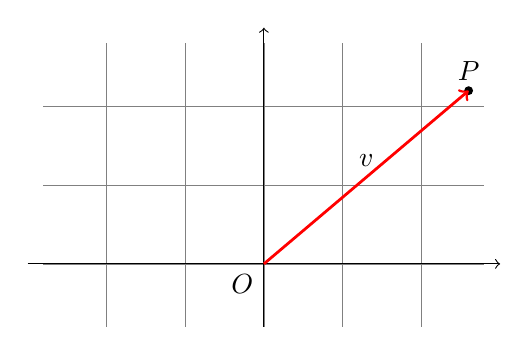
\begin{tikzpicture}[scale=2]
  \clip (-1.5,-0.4) rectangle (1.5,1.5);
  \draw[step=.5cm,gray,very thin] (-1.4,-1.4) grid (1.4,1.4);
  \draw[->] (-1.5,0) -- (1.5,0);
  \draw[->] (0,-1.5) -- (0,1.5);
  \fill (1.3,1.1) circle (0.8pt) node[above]{$P$};
  \draw[red,line width=1pt, ->] (0,0) node[below left, black] {$O$} -- (1.3,1.1) node[midway, above, black] {$\ve v$};    
\end{tikzpicture}

  \caption{Vettore $\ve v$ applicato nell'origine che individua il punto $P$.}
\end{figure}
\section{\index{versore}Versori e \index{coordinate}coordinate}
I versori sono vettori della base ortonormale di $\field{R}^3$ (lo spazio) considerato con il prodotto scalare canonico. In parole povere sono sono vettori di modulo unitario ortogonali a due a due. Solitamente si indicano con $\ver i$, $\ver j$ e $\ver k$ i versori applicati nell'origine, nella direzione degli assi cartesiani del sistema di riferimento. Le loro coordinate sono\footnote{quando si scrive che $\ve v=(a,b,c)$ l'uguaglianza significa che che fissata una base il vettore è rappresentato dalle sue coordinate $(a,b,c)$, ma vettori e coordinate non sono la stessa cosa, per esempio se si fa un cambiamento di base il vettore non cambia, ma le sue coordinate sì.}:
\[
\ver \imath=\left(\begin{array}{c} 1\\0\\0\\ \end{array}\right)\qquad
\ver \jmath=\left(\begin{array}{c} 0\\1\\0\\ \end{array}\right)\qquad
\ver k=\left(\begin{array}{c} 0\\0\\1\\ \end{array}\right)
\]

Poiché i versori formano una base ogni vettore può essere espresso come una loro combinazione lineare, i coefficienti sono le coordinate\footnote{come già accennato i due simboli di uguaglianza hanno significati diversi, il primo è una vera uguaglianza, il secondo vuol dire che fissata una base, il vettore è rappresentato da quelle coordinate.}:
\[
\ve v=v_x\ve i+v_y\ve j+v_z\ve k=\left(
\begin{array}{c}
v_x\\v_y\\v_z\\
\end{array}\right)
\]
\section{Individuazione vettori}
\begin{figure}[htbp]
 \centering
 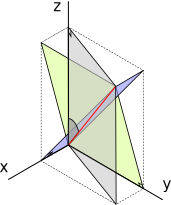
\includegraphics{immagini/fisica1/vettore_geometrico}
 % vettore_geometrico.pdf: 161x165 pixel, 72dpi, 5.68x5.82 cm, bb=0 0 161 165
 \caption{l'angolo evidenziato è l'angolo $\alpha$ tra il vettore e l'asse $z$. Quest'angolo appartiene al piano individuato dal vettore e dall'asse $z$ (in grigio).}
\end{figure}
I vettori si possono individuare in un sistema di riferimento per via geometria o per via analitica. Individuando un vettore per via geometrica si indica il modulo, e gli angoli che il vettore forma con gli assi cartesiani. Nello spazio:
\[
\left\{
\begin{array}{l}
|\ve v|\\
\alpha,\beta,\gamma
\end{array}\right. \qquad \text{con}\qquad \cos^2 \alpha+\cos^2 \beta + \cos^2
\gamma=1
\]
Notiamo che gli angoli $\alpha$, $\beta$ e $\gamma$ non sono indipendenti, possiamo ricavarne uno in funzione degli altri; quindi un vettore sarà descritto da tre informazioni, per esempio $|\ve v|$, $\alpha$, $\beta$.

Per via analitica invece bisogna indicare le componenti del vettore rispetto alla base $\{\ve i, \ve j, \ve k\}$: $\left(
\begin{array}{l}
v_x\\v_y\\v_z
\end{array}\right)
$.
\subsection{Passaggio da individuazione geometrica a individuazione analitica}
\[
\left\{
\begin{array}{l}
v_x=|\ve v|\cos\alpha\\
v_y=|\ve v|\cos\beta\\
v_z=|\ve v|\cos\gamma
\end{array}
\right. \qquad \qquad \left\{
\begin{array}{l}
|\ve v|^2=v_x^2+v_y^2+v_z^2\\
\cos\alpha=\cfrac{v_x}{|\ve v|}\\
\cos\beta=\cfrac{v_y}{|\ve v|}\\
\cos\gamma=\cfrac{v_z}{|\ve v|}
\end{array}
\right.
\]


\section{Operazioni tra i vettori}

\subsubsection{Vettore inverso}
Il vettore inverso ha stesso modulo del vettore, stessa direzione,
ma verso opposto.
\[
-\ve v=-(v_x\ve i+v_y\ve j+v_z \ve k)=-v_x\ve i-v_y\ve
j-v_z\ve k
\]
Naturalmente ogni vettore ha inverso e la loro somma è nulla e $-\ve 0=\ve 0$.

\subsubsection{Somma}
La somma di due vettori è il vettore che ha come componenti la somma delle componenti. Dal punto di vista grafico equivale a usare la regolare del parallelogramma:
\begin{multline*}
\ve a+\ve b=(a_x\ve i+a_y\ve j+a_z \ve k)+(b_x\ve
i+b_y\ve j+b_z\ve k)=\\
=(a_x+b_x)\ve i+(a_y+b_y)\ve
j+(a_z+b_z)\ve k
\end{multline*}

\begin{figure}[htbp]
  \centering
  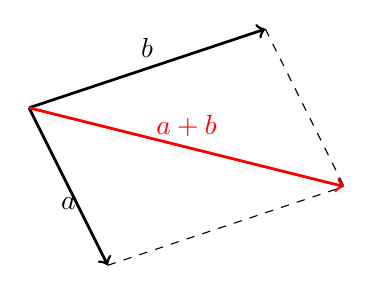
\begin{tikzpicture}[scale=1]
\draw[line width=1pt, ->] (3,7) -- (4,5) node[midway, below] {$\ve a$};
\draw[line width=1pt, ->] (3,7) -- (6,8) node[midway, above] {$\ve b$};
\draw[dashed] (4,5) -- (7,6);
\draw[dashed] (6,8) -- (7,6);
\draw[line width=1pt, red, ->] (3,7) -- (7,6) node[midway, above] {$\ve a + \ve b$};
\end{tikzpicture}

  \caption{Regola del parallelogramma.}
\end{figure}

\subsubsection{Differenza} La differenza di due
vettori è la somma del primo con l'inverso del secondo. Graficamente $\ve a-\ve b$ è il vettore che congiunge $\ve b$ ad $\ve a$.
\subsubsection{Prodotto per uno scalare}
Per via geometrica il prodotto scalare di un vettore per uno scalare corrisponde al vettore con stessa direzione, con modulo moltiplicato per il valore assoluto dello scalare e verso invertito se lo scalare è negativo.
\[\forall h \in \field{R}\qquad h\ve a=h(a_x\ve i+a_y\ve j+a_z\ve k)=ha_x\ve i+ha_y\ve j+ha_z\ve k\]
\subsubsection{\index{prodotto!scalare}Prodotto scalare}
Il prodotto scalare usato in fisica è il prodotto scalare canonico della geometria in $\field{R}^3$ rispetto alla base canonica $\{\ve i,\ve j,\ve k\}$:
\[\left(\ve{x},\ve{y}\right)=\ve{x}^T\cdot\ve{y}=(x_1y_1+x_2y_2+x_3y_3)\]
\[p_s=|\ve a||\ve b| \cos \alpha\]
 con $\alpha$ l'angolo compreso tra i due vettori. Da qui si deduce che $\ve i \cdot \ve i=1$, $\ve i
\cdot \ve j=0$, ecc., che due vettori ortogonali hanno prodotto scalare nullo e che due vettori hanno prodotto scalare massimo quando sono paralleli.
\[p_s=\ve a \cdot \ve b=(a_x\ve i+a_y\ve j+a_z\ve k)\cdot(b_x\ve
i+b_y\ve j+b_z\ve k)=a_xb_x+a_yb_y+a_zb_z\]
\subsubsection{\index{prodotto!vettoriale}Prodotto Vettoriale}
Matematicamente il prodotto vettoriale non è facile da definire. Esso restituisce un vettore che ha direzione ortogonale al piano individuato dai due vettori, verso ricavabile dalla regola della mano destra, e modulo:
\[|\ve p_v|=ab\sin \alpha\] con $\alpha$ angolo tra i due vettori\footnote{è molto semplice ricordarsi la formula del prodotto vettoriale, basta ciclare sulle variabili. Per esempio la componente $x$ del prodotto vettoriale è $a_yb_z-a_zb_y$ in cui l'ordine è $x$ (la componente) e poi $y$, $z$, seguito dalla sottrazione al contrario (è antisimmetrico)}.


\begin{align*}
\ve p_v&=\ve a \wedge \ve b=\ve a \times \ve b=(a_x\ve i+a_y\ve j+a_z\ve k)\wedge(b_x\ve
i+b_y\ve j+b_z\ve k)\\
&=(a_yb_z-a_zb_y)\ve i+(a_zb_x-a_xb_z)\ve j+(a_xb_y-a_yb_x)\ve k
\end{align*}

Il prodotto scalare può essere calcolato come determinante di una matrice $3\times 3$:
\[\ve p_v=
\left| \begin{array}{ccc} \ve i & \ve j & \ve k\\
a_x & a_y & a_z\\
b_x & b_y& b_z
 \end{array} \right|\]

Il prodotto vettoriale è antisimmetrico cioè $\ve a \wedge \ve
b=-\left(\ve b \wedge \ve a\right)$. Il modulo del prodotto
vettoriale è l'area del parallelogramma avente come lati i due
vettori.

Il prodotto vettoriale è dipendente dalla scelta del sistema di riferimento. In particolare il verso del prodotto vettoriale segue la regola della mano destra se il sistema di riferimento è destrogiro, altrimenti il verso risulta opposto. Per questo il prodotto vettoriale è chiamato pseudovettore. In natura le grandezze osservabili non devono dipendere dalla scelta dell'orientazione (chiralità) degli assi cartesiani. Per convenzione si sceglie un sistema di riferimento destrogiro.
\begin{figure}[htbp]
\centering
\subfigure[destrogiro]{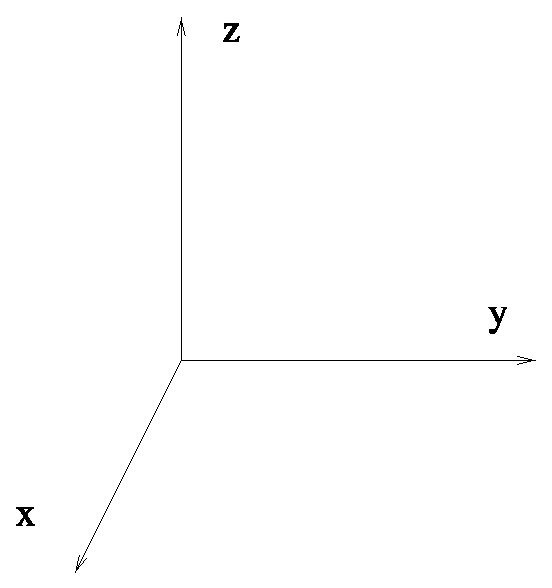
\includegraphics[scale=0.5]{immagini/fisica1/sistema_destrogiro}}
\subfigure[sinistrogiro]{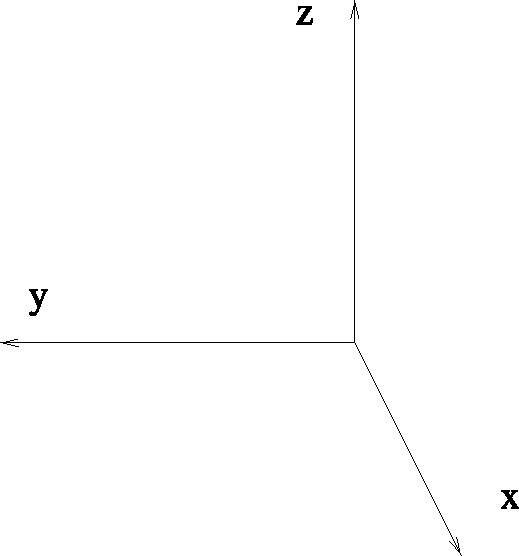
\includegraphics[scale=0.5]{immagini/fisica1/sistema_sinistrogiro}}
\end{figure}

\subsubsection{\index{prodotto!misto}Prodotto Misto}
Il prodotto misto è definito come:
\[p_m=\ve c\cdot\left(\ve a \wedge \ve b\right)\]
Esso è uguale all'area del parallelepipedo avente come spigoli i
vettori \mbox{$\ve a$, $\ve b$, $\ve c$.}

\subsubsection{\index{derivata!di un vettore}Derivata di un vettore}
La derivata di un vettore è la derivata delle coordinate per i rispettivi versori, (i versori sono costanti). Per esempio la derivata della velocità rispetto al tempo è:
\[\frac{\ud\ve v}{\ud t}=\frac{\ud v_x}{\ud t}\ve i+\frac{\ud v_y}{\ud t}\ve j+\frac{\ud v_z}{\ud t}\ve k\]

\subsubsection{\index{gradiente}Gradiente}
\label{gradiente}
Il gradiente di uno scalare è definito come:
\[
\grad V(x,y,z)=\ve\nabla V(x,y,z)=\frac{\partial V}{\partial x}\ver i + \frac{\partial V}{\partial y}\ver j +\frac{\partial V}{\partial z}\ver k +
\]
dove $\ve\nabla$ è un operatore definito come:
\[
\ve\nabla=\left(\frac{\partial}{\partial x},\frac{\partial}{\partial y},\frac{\partial }{\partial z}\right)
\]
con questo operatore abbiamo il divertimento di scrivere le nostre formule per esempio in questo modo:

\[
\ve F=-\ve\nabla U
\]
invece di:
\[
\ve F=-\left(\frac{\partial U}{\partial
x}\ve i+\frac{\partial U}{\partial y}\ve j+\frac{\partial
U}{\partial z}\ve k\right)
\]

\chapter{Cinematica}
\minitoc
\section{\index{posizione}Vettore posizione}
\begin{Def}[vettore posizione]
Fissato un sistema di riferimento cartesiano\footnote{per semplicità quasi sempre si parlerà del piano piuttosto che dello spazio, ma i risultati sono del tutto analoghi} $Oxy$ il vettore che congiunge l'origine con un punto $P$ è il \index{vettore!posizione}vettore posizione $\ve r$ che individua $P$ in quel sistema di riferimento.
\end{Def}
Poiché il punto può spostarsi nel tempo $\ve r$ sarà funzione del tempo $\ve r=\ve r(t)$ e descriverà al variare del tempo tutte le posizioni occupate da $P$ cioè la sua traiettoria\index{traiettoria}.

\begin{figure}[htbp]
\centering
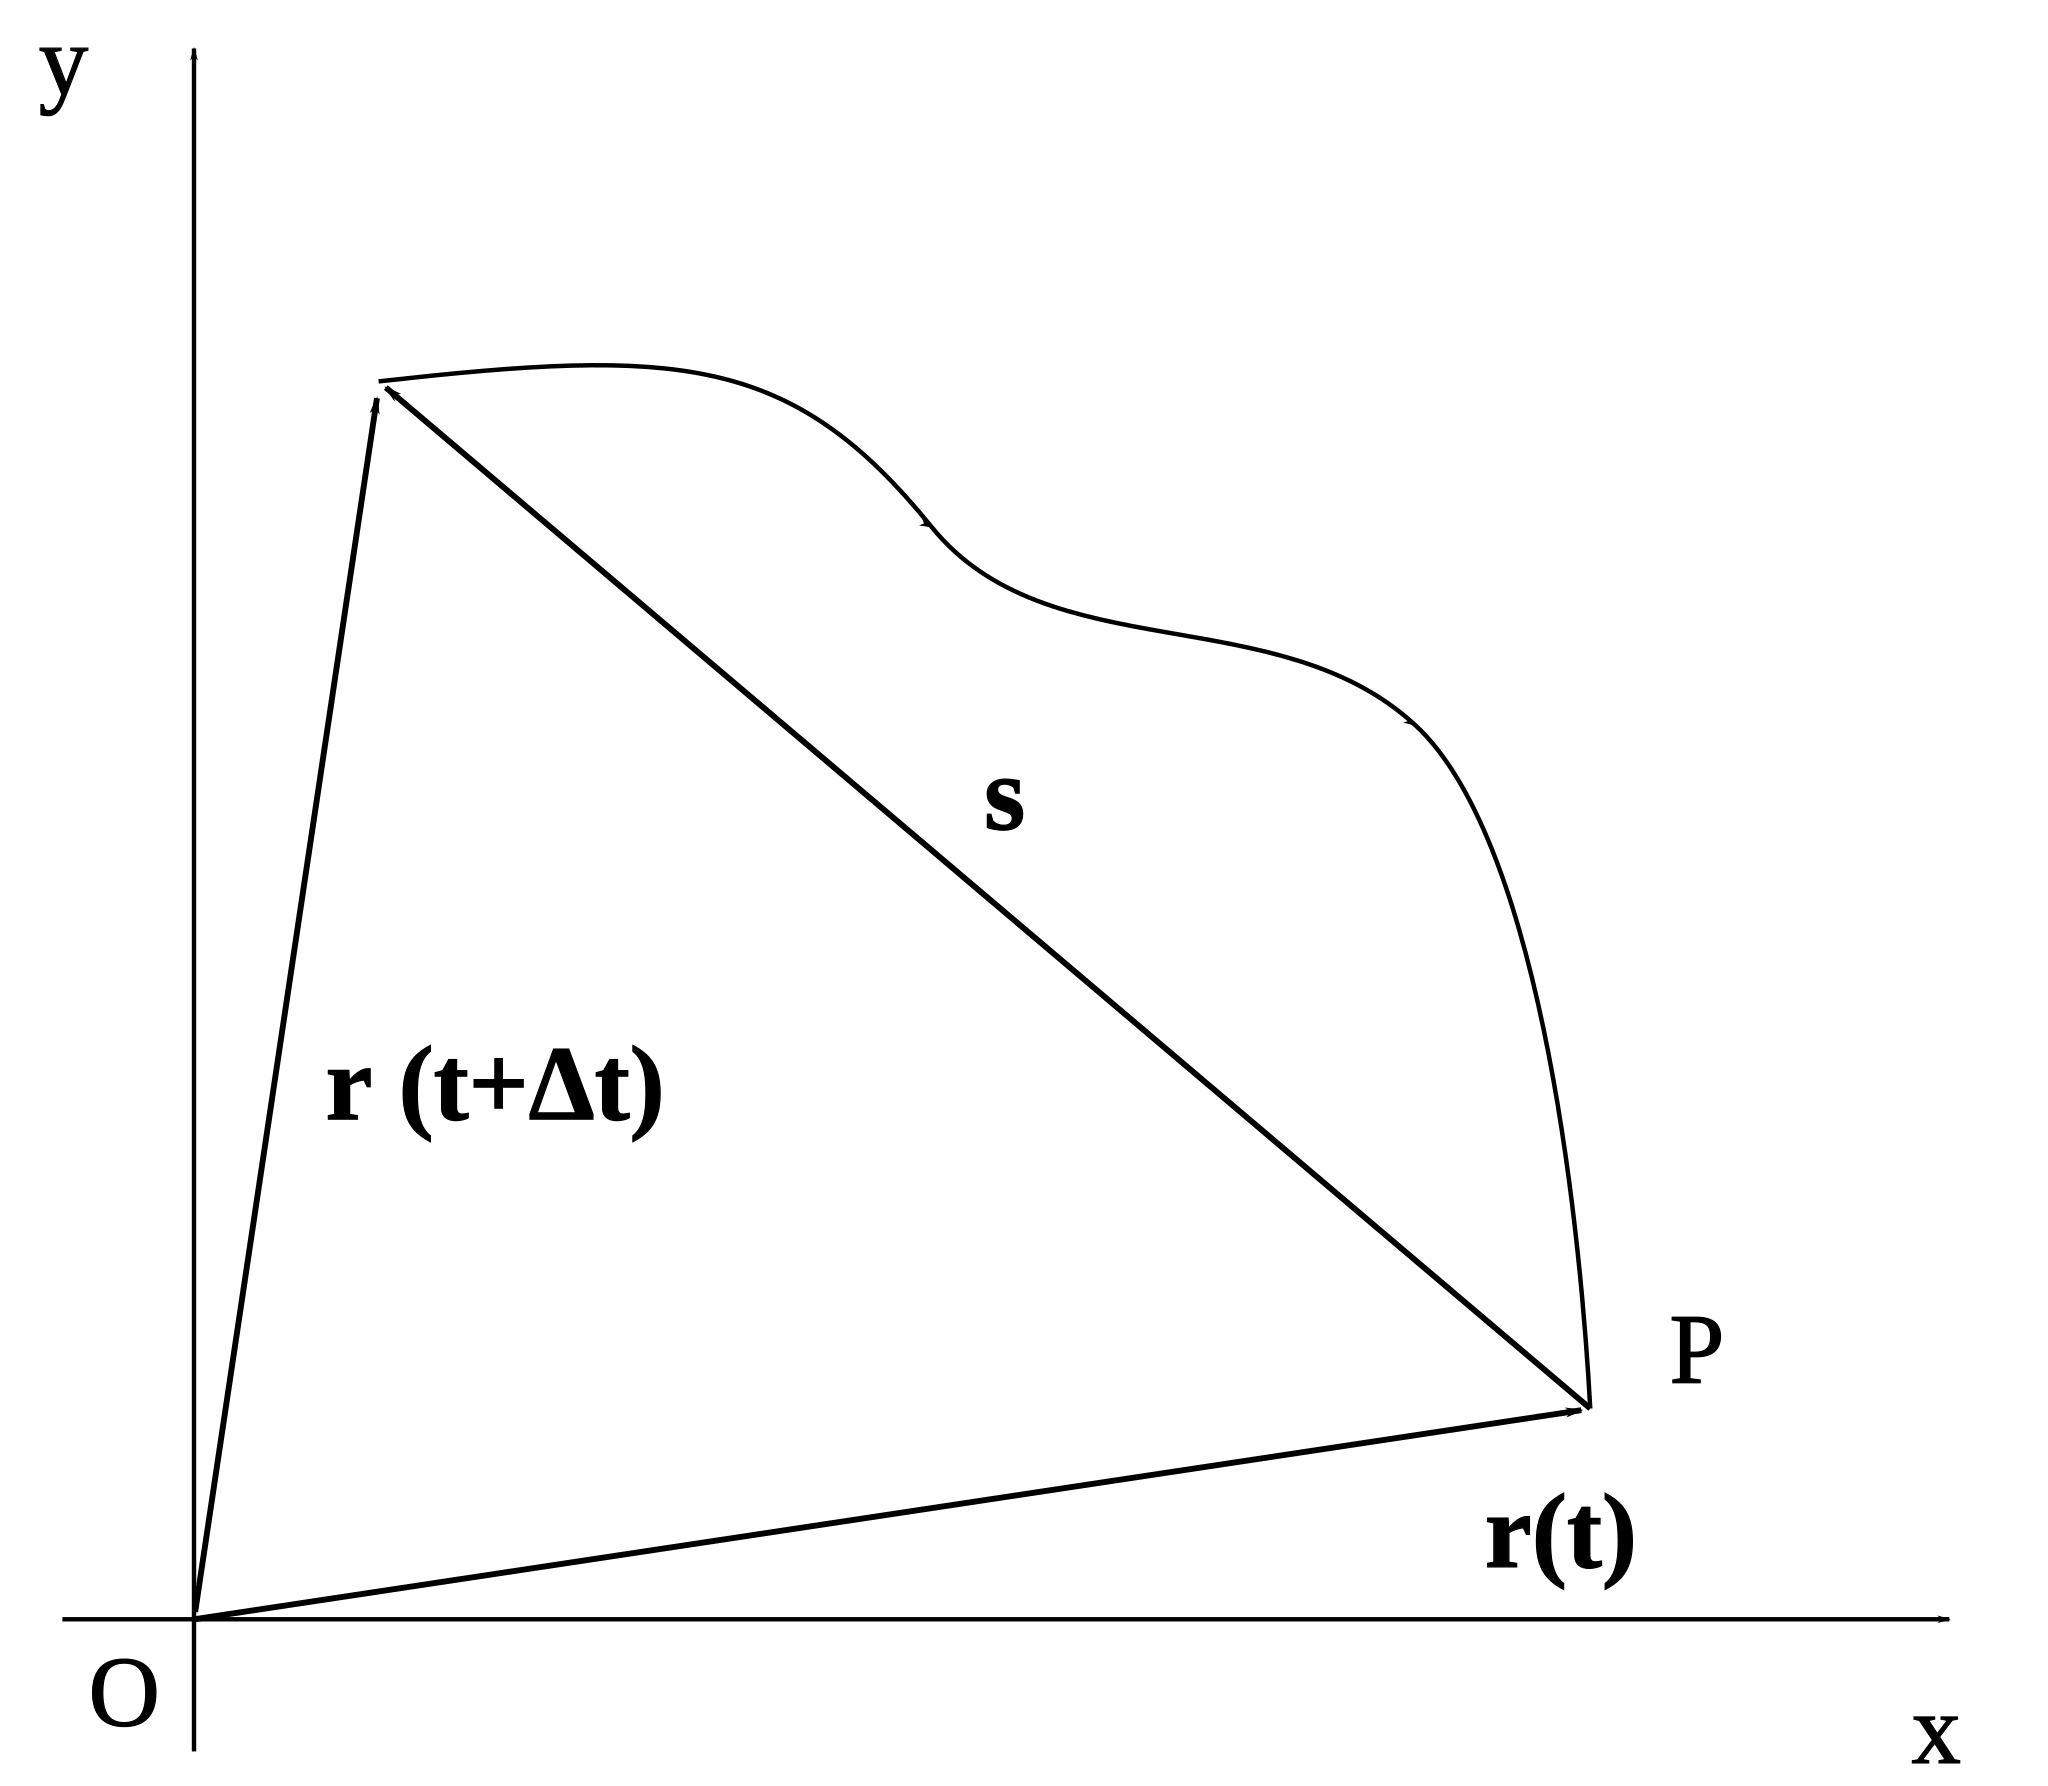
\includegraphics[scale=0.7]{immagini/fisica1/vettore_posizione}
\caption{vettore posizione e spostamento.}
\end{figure}
\subsection{Vettore spostamento}
\begin{Def}[vettore spostamento]
Il \index{vettore!spostemento} vettore spostamento è la variazione (differenza) del vettore posizione tra due istanti diversi:
\begin{align*}
\ve s\left(t,t+\Delta t\right)&=\Delta \ve r(t,t+\Delta t)\\
&=\ve r\left(t+\Delta t\right)-\ve r\left(t\right)=x\left(t+\Delta t\right)\ve i+y\left(t+\Delta t\right)\ve j-x\left(t\right)\ve i-y\left(t\right)\ve j\\
&=\left[x(t+\Delta t)-x(\Delta t)\right]\ve i+[y(t+\Delta t)-y(t)]\ve j=\Delta x\ve i+\Delta y \ve j
\end{align*}
\end{Def}
\section{\index{velocità}Vettore velocità}
\begin{Def}[\index{velocità!media}Velocità Media]
\[\ve v_m(t,t+\Delta t)=\frac{\Delta\ve r(t,t+\Delta t)}{\Delta
t}=\frac{1}{\Delta t}\{\Delta x\ve i+\Delta y\ve
j\}=\frac{\Delta x}{\Delta t}\ve i+\frac{\Delta y}{\Delta t}\ve
j\]
\end{Def}
\begin{Def}[\index{velocità!istantanea}Velocità Istantanea]
\[\ve v(t)=\lim_{\Delta t\rightarrow 0}\ve v_m(t,t+\Delta t)=\lim_{\Delta t\rightarrow 0} \frac{\Delta\ve r}{\Delta t}(t)={\left.\frac{\ud \ve r}{\ud t}\right|_t}=\left.\frac{\ud x}{\ud t}\right|_t\ve i+\left.\frac{\ud y}{\ud t}\right|_t\ve j\]
\end{Def}
Si noti che la norma della derivata non è la derivata della norma:
\[\norm{\ve v}=\norm{\frac{\ud\ve r}{\ud t}}\neq\frac{\ud}{\ud t}\norm{\ve r}\]
\begin{Def}[\index{velocità!scalare}Velocità Scalare]
\[v_s=\frac{\text{spazio totale percorso}}{\Delta t}\]
\end{Def}
\section{\index{accelerazione}Vettore accelerazione}
\begin{Def}[accelerazione istantanea]
\[\ve a=\frac{\ud \ve v}{\ud t}={\frac{\ud^2 \ve r}{\ud t^2}}\]
\end{Def}
\section[Moto rettilineo uniforme]{\index{moto!rettilineo uniforme}Moto rettilineo uniforme\protect\footnote{usiamo sempre condizioni iniziali implicite, del tipo $t_0=0$, $\ve r(0)=\ve r_0$, $\ve v(0)=\ve v_0$}}
\begin{Def}[moto rettilineo uniforme]
\[\ve v=\overrightarrow\const\]
\end{Def}
\[\ud\ve r=\ve v\,\ud t\qquad\int_{\ve r_0}^{\ve r}\ud\ve r=\int_0^t\ve v\,\ud t \qquad \ve r-\ve r_0=\ve v t\]
\begin{eqimp}{equation}
\ve r=\ve v t+\ve r_0
\end{eqimp}
\section{\index{moto!uniformemente accelerato}Moto uniformemente accelerato}
\begin{Def}[moto uniformemente accelerato]
\[\ve a=\overrightarrow{\const}\]
\end{Def}
\[\ve a\,\ud t=\ud \ve v\qquad\int_0^t\ve a\,\ud t=\int_{\ve v_0}^{\ve v}\ud \ve v\qquad\ve a t=\ve v-\ve v_0\]
\begin{eqimp}{equation}
\ve v=\ve a t+\ve v_0
\label{vt_01}
\end{eqimp}
\[\ve v=\ve a t+\ve v_0=\frac{\ud \ve r}{\ud t}\]
\[\ud \ve r=\left(\ve a t+\ve v_0\right)\ud t\qquad\int_{\ve r_0}^{\ve r}\ud \ve r=\int_0^t\left(\ve a t+\ve v_0\right)\ud t\qquad\ve r-\ve r_0=\frac{1}{2}\ve a t^2+\ve v_0 t\]
\begin{eqimp}{equation}
\ve r=\frac{1}{2}\ve a t^2+\ve v_0 t+\ve r_0
\label{vt_02}
\end{eqimp}
\subsection{Velocità in funzione dello spazio}
In certi casi può risultare molto comoda la formula relativa al
moto uniformemente accelerato scritta in questo modo:
\begin{equation}
v^2-v_0^2=2a(r-r_0)
\label{vt_03}
\end{equation}
che vale solo nel caso unidimensionale\footnote{nel caso unidimensionale le \eqref{vt_01} e la \eqref{vt_02} si scrivono come:
\begin{equation}
v(t)=at+v_0\qquad r(t)=\frac{1}{2}at^2+v_0t+r_0
\end{equation}
eliminiamo il tempo per trovare $v(r)$: ricaviamo $t$ dalla prima e sostituiamolo nella seconda, semplifichiamo e otteniamo la \eqref{vt_03}}.
\section{\index{moto!circolare!uniforme}Moto circolare uniforme}
Per moto circolare uniforme si intende quel moto su traiettoria
circolare in cui il modulo del vettore velocità rimane costante
nel tempo (mentre la sua direzione varia ed è sempre tangente
alla circonferenza). Definiamo la velocità angolare\index{velocità!angolare}\index{omega@$\omega$|see{velocità angolare}}: $\omega=\frac{\ud\theta}{\ud t}$ e l'accelerazione angolare\index{accelerazione!angolare}\index{alpha@$\alpha$|see{accelerazione angolare}} $\alpha=\frac{\ud \omega}{\ud t}$; in realtà possono essere definiti come vettori.
\[\norm{\ve v}=\const\]
\[\text{scegliamo $\ve r(t=0)=\ve r_0$}:\left\{
\begin{array}{l}
x=R\\
y=0\\
\end{array}\right.\]
\[\ve r=R\cos\theta\ve i+R\sin\theta\ve j\]
\[\theta=\frac{\text{arco}}{\text{raggio}}=\frac{vt}{R}=\omega t\qquad\omega=\dot\theta=\frac{v}{R}=\const\]
\[\ve r=R\cos(\omega t)\ve i+R\sin(\omega t)\ve j\]
\[\ve v=\frac{\ud \ve r}{\ud t}=-R\omega\sin(\omega t)\ve
i+R\omega\cos(\omega t)\ve j\]
\begin{align*}|\ve v|^2&=v_x^2+v_y^2=R^2\omega^2\sin^2(\omega
t)+R^2\omega^2\cos^2(\omega t)\\
&=R^2\omega^2\left(\sin^2\left(\omega t\right)+\cos^2\left(\omega
t\right)\right)=R^2\omega^2
\end{align*}
\[v=\omega R\]
\[\ve v\cdot\ve r=0\Rightarrow\ve v\bot\ve r\]
\[\ve v\cdot\ve r=v_xx+v_yy=-R\omega\sin(\omega t)R\cos(\omega t)+R\omega\cos(\omega t)R\sin(\omega t)=0\]
\begin{align*}
\ve a&=\frac{\ud\ve v}{\ud t}=-R\omega^2\cos(\omega t)\ve
i-R\omega^2\sin(\omega t)\ve j\\
&=-R\omega^2\left(\cos\left(\omega t\right)\ve i+
\sin\left(\omega t\right)\ve j\right)=-\omega^2\ve r
\end{align*}
\[|\ve a|^2=R^2\omega^4\cos^2(\omega t)+R^2\omega^4\sin^2(\omega
t)=R^2\omega^4\]
\[a=\omega^2R=\omega v=\frac{v^2}{R}\]
\section{\index{moto!circolare}Moto circolare}
\begin{figure}[htbp]
\centering
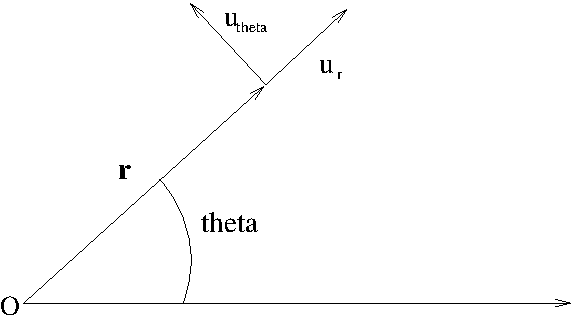
\includegraphics[scale=1]{immagini/fisica1/CorPol}
\caption{\index{coordinate!polari}Coordinate polari.}
\end{figure}
\[\ve r=R\ve u_r\]
\[
\left\{\begin{array}{ll}
\ve u_r=\cos\theta(t)\ve i+\sin\theta(t)\ve j\\
\ve u_\theta=-\sin\theta(t)\ve i+\cos\theta(t)\ve j
\end{array}\right.
\]
\[\frac{\ud\ve u_\theta}{\ud t}=-\dot{\theta}\cos\theta\ve i-\dot{\theta}\sin\theta\ve j=-\dot{\theta}\ve u_r\]
\begin{align*}
\ve v&=\frac{\ud \ve r}{\ud t}=\frac{\ud\left(R\ve
u_r\right)}{\ud t}=R\frac{\ud \ve u_r}{\ud
t}\\
&=R\left(-\dot\theta\sin\theta\ve i+\dot\theta\cos\theta\ve
j\right)=R\dot\theta\ve u_\theta
\end{align*}
\[\ve a=\frac{\ud\ve v}{\ud t}=\frac{\ud\left(R\dot\theta\ve
u_\theta\right)}{\ud t}=R\ddot\theta\ve
u_\theta+R\dot\theta\frac{\ud\ve u_\theta}{\ud
t}=R\ddot\theta\ve u_\theta-R\dot\theta^2\ve u_r\]


\section{\index{moto!in coordinate polari}Moto qualsiasi in coordinate polari}
\[\ve r(t)=r\ve u_r\]
\[\ve u_r=\cos\theta\ve i+\sin\theta\ve j\qquad \ve u_\theta=-\sin\theta\ve i+\cos\theta\ve j\]
\[\frac{\ud\ve u_r}{\ud t}=-\dot\theta\sin\theta\ve
i+\dot\theta\cos\theta\ve j=\dot\theta\left(-\sin\theta\ve
i+\cos\theta\ve j\right)=\dot\theta\ve u_\theta\]
\[\frac{\ud\ve u_\theta}{\ud t}=-\dot\theta\cos\theta\ve
i-\dot\theta\cos\theta\ve j=-\dot\theta\left(\cos\theta\ve
i+\sin\theta\ve j\right)=-\dot\theta\ve u_r\]
\[\ve v=\frac{\ud\ve r}{\ud t}=\dot r\ve u_r+r\frac{\ud\ve
u_r}{\ud t}=\dot r\ve u_r+r\dot\theta\ve u_\theta\]
\[\ve a=\frac{\ud\ve v}{\ud t}=\ddot r\ve u_r+\dot
r\dot\theta\ve u_\theta+\dot r\dot\theta\ve
u_\theta+r\ddot\theta\ve u_\theta-r\dot\theta^2\ve u_r=\ve
u_r\left(\ddot r-r\dot\theta^2\right)+\ve u_\theta\left(2\dot
r\dot\theta+r\ddot\theta\right)\]

 I vettori velocità e accelerazione vengono scomposti in due
componenti:
\begin{enumerate}
\item[--] \index{velocità!radiale}Velocità radiale: $v_r=\dot r$
\item[--] \index{velocità!perpendicolare}Velocità perpendicolare: $v_\theta=r\dot\theta$
\item[--] \index{accelerazione!radiale}Accelerazione radiale: $a_r=\ddot r-r\dot\theta^2$
\item[--] \index{accelerazione!perpendicolare}Accelerazione perpendicolare: $a_\theta=2\dot r\dot\theta+r\ddot
\theta$
\end{enumerate}
\section{\index{moto!armonico}Moto armonico}
\begin{figure}[htbp]
 \centering
 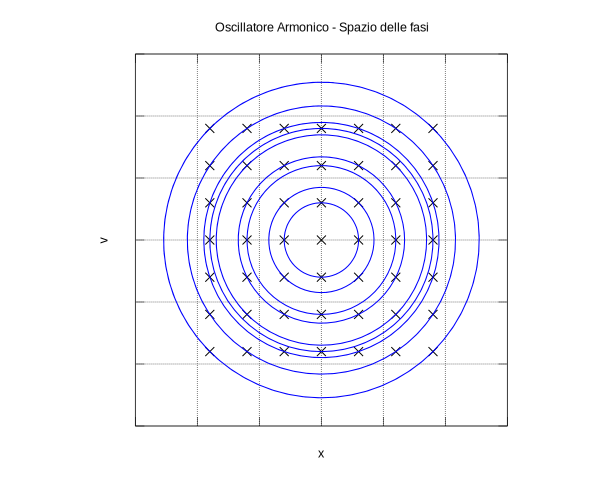
\includegraphics[scale=0.6]{immagini/fisica1/oscillatore_fase}
 % oscillatore_fase.: 480x384 pixel, 72dpi, 16.93x13.55 cm, bb=0 0 480 384
 \caption{Traiettorie nello spazio delle configurazioni dell'oscillatore armonico a partire da diverse condizioni iniziali.}
\end{figure}
Il moto armonico è un moto con equazione differenziale:
\begin{eqimp}{equation}
\ddot x=-\omega^2 x
\end{eqimp}
la cui soluzione è:
\[x=A\sin(\omega t+\varphi)\]
derivando si ottiene
\[v=\frac{\ud x}{\ud t}=A\omega\cos(\omega t+\varphi)\]
\[a=\frac{\ud v}{\ud t}=-A\omega^2\sin(\omega t+\varphi)\]
ovviamente risulta che: $a = -\omega^2 x=\ddot x$.
Per esempi (pendoli, molle) vedi sezione \ref{armonico} a pagina \pageref{armonico}.
\subsection{Moto armonico smorzato\index{moto!armonico!smorzato}}
\begin{figure}
 \centering
 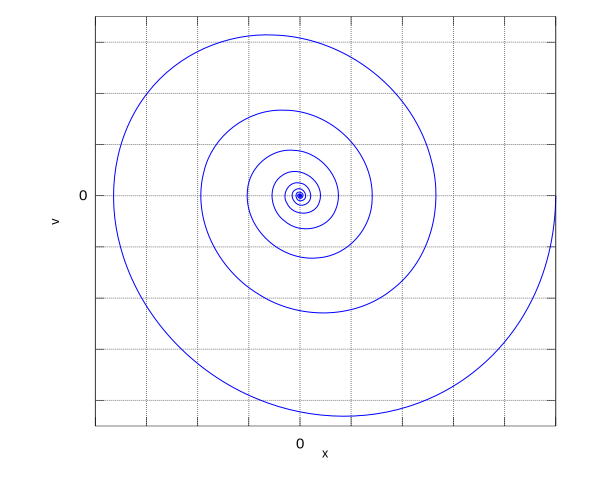
\includegraphics[scale=0.6]{immagini/fisica1/oscillatore_smorzato_fase}
 % oscillatore_smorzato_fase.pdf: 480x384 pixel, 72dpi, 16.93x13.55 cm, bb=0 0 480 384
 \caption{Traiettorie nello spazio delle configurazioni dell'oscillazione smorzato con coefficiente di attrito debole.}
\end{figure}
Introduciamo nel moto armonico una forza smorzatrice, per esempio una forza d'attrito che varia con la velocità:
\[F=-\gamma \frac{\ud x}{\ud t}\]
\[m\ddot x=-kx-\gamma\dot x\qquad m\ddot x+\gamma\dot x+kx=0\]
$\tau=\frac{m}{\gamma}$ è un tempo, la frequenza del moto armonico non smorzato è $\frac{k}{m}=\omega_0^2$
\[\ddot x+\frac{\gamma}{m}\dot x+\frac{k}{m}x=0\qquad \ddot x+\frac{1}{\tau}\dot x+\omega_0^2x=0\]
se $\tau=\infty$ allora il moto non è più smorzato.

Una soluzione è:
\[x(t)=e^{st}\]
\[\dot x(t)=sx(t)\qquad \ddot x(t)=s^2x(t)\]
\[s^2x(t)+\frac{1}{\tau}sx(t)+\omega_0^2x(t)=0\]
\[s_{1/2}=\dfrac{-\dfrac{1}{\tau}\pm\sqrt{\dfrac{1}{\tau^2}-4\omega_0^2}}{2}=-\frac{1}{2\tau}\pm\sqrt{\frac{1}{4\tau^2}-\omega_0^2}\]
quindi la soluzione generale è una combinazione lineare delle soluzioni:
\[
 x(t)=A_1e^{s_1t}+A_2e^{s_2t}
\]
a seconda che le radici del polinomio siano reali o complesse si possono distinguere due casi:
\begin{description}
\item[attrito forte]
\[\beta=\frac{1}{4\tau^2}-\omega_0^2>0\qquad\tau<\frac{1}{2\omega_0}\qquad\gamma>2\sqrt{km}\]
\[s_{1/2}=-\frac{1}{2\tau}\pm\beta\qquad\text{radici reali e}<0\]
\[x(t)=A_1e^{s_1t}+A_2e^{s_2t}\]
\item[attrito debole]
\[\frac{1}{4\tau^2}-\omega_0^2<0\qquad \tau>\frac{1}{2\omega_0}\qquad\gamma<2\sqrt{km}\]
\[s_{1/2}=\dfrac{-\dfrac{1}{\tau}\pm\sqrt{\dfrac{1}{\tau^2}-4\omega_0^2}}{2}=-\frac{1}{2\tau}\pm i\omega\]
\begin{align*}x(t)&=A_1e^{s_1it}+A_2e^{s_2it}=A_1e^{-\frac{t}{2\tau}-i\omega t}+A_2e^{-\frac{t}{2\tau}+i\omega t}=\\
&=e^{-\frac{t}{2\tau}}\left(A_1e^{-i\omega t}+A_2e^{i\omega t}\right)=A e^{-\frac{t}{2\tau}}\sin(\omega t +\varphi)\end{align*}
quindi è un moto armonico con frequenza $\omega=\sqrt{\omega_0-\frac{1}{4\tau^2}}$ la cui ampiezza diminuisce con un fattore frenante $e^{-\frac{t}{2\tau}}$.\footnote{Il caso critico in cui ci siano due radici coincidenti è tralasciato poiché puntiforme}
\end{description}

\section{\index{trasformazioni!di Galileo}Trasformazioni di Galileo}
Le trasformazioni di Galileo sono equazioni valide nella meccanica classica che consentono di descrivere le coordinate di un sistema rispetto alle di coordinate di un altro sistema che si muove di moto rettilineo uniforme rispetto al primo. Un sistema è detto inerziale se vale la prima legge di Newton. Se in un sistema è inerziale allora un altro sistema è inerziale se e solo se si muove di motto rettilineo uniforme rispetto al primo.
\newline

Primo osservatore ``fermo'':$\qquad O\quad\ve r\quad\;\ve
v\quad\;\ve a$

Secondo osservatore in moto:$\quad O'\quad\!\ve r\,'\quad\!\ve
v\,'\quad\!\ve a\,'$

In meccanica classica si assume:$\quad t=t'$

$\ve u$ velocità di trascinamento: \index{velocità!relativa}velocità di $O'$ rispetto ad $O$.
\begin{legge}
$\ve r(t)=\overrightarrow{\left(O'-O\right)}+\ve r\,'=\ve u
t+\ve r\,'$
\end{legge}
\begin{legge}[composizione delle velocità]
\index{composizione delle velocità}
\[\ve v=\frac{\ud\ve r}{\ud t}=\frac{\ud}{\ud t}\left(\ve u
t+\ve r\,'\right)=\frac{d}{\ud t}\left(\ve u
t\right)+\frac{\ud\ve r\,'}{\ud t}=\ve u+\frac{\ud\ve r\,'}{\ud
t'}=\ve u+\ve v\,'\]
velocità assoluta = velocità relativa + \index{velocità!di trascinamento}velocità di trascinamento
\end{legge}
\begin{legge}[invarianza dell'accelerazione]
\[\ve a=\frac{\ud \ve v}{\ud t}=\frac{\ud}{\ud t}(\ve u+\ve
v\,')=0+\frac{\ud \ve v\,'}{\ud t}=\frac{\ud \ve v\,'}{\ud
t'}=\ve a'\]
L'accelerazione quindi è invariante
\end{legge}
\[\left\{\begin{array}{ll}
\ve r=\ve r\,'+\ve u t&\text{trasformate di Galileo}\\
\ve v=\ve u+\ve v\,'&\text{somma delle velocità}\\
\ve a=\ve a\,'&\text{invarianza dell'accelerazione}\\
t=t'&\text{ipotesi del tempo assoluto}\\
\end{array}\right.\]
Esse valgono nell'ipotesi che se $t=0=t'$ allora $\ve r\,'=\ve r$.
Non esiste un sistema di riferimento assoluto.
\begin{Es}[lancio del sasso]
 Consideriamo due sistemi inerziali $O$ e $O'$. $O$ veda $O'$ muoversi lungo l'asse $x$ con velocità $\ve w$. Siano gli assi $y$ e $z$ uguali nei due sistemi. $O$ lancia un sasso verso l'alto, le equazioni del moto per il sasso visto da $O$ sono:
 \begin{gather*}
  x(t) = x_0\\
  y(t) = -\frac{1}{2}gt^2 + v_0 t
 \end{gather*}
 la traiettoria in questo caso è un segmento verticale con gli estremi in $(x_0,0)$ e $(x_0,\frac{v_0^2}{2g})$. Nel sistema $O'$ invece questo moto diventa:
 \begin{gather*}
  x'(t) = x(t) - w t = x_0 - wt\\
  y(t) = -\frac{1}{2}gt^2 + v_0 t
 \end{gather*}
 si noti che $v_0$ è sempre lo stesso nei due sistemi. Eliminando il tempo: $t = (x_0-x') /w$ si ottiene l'equazione di una parabola il cui vertice è ad una altezza uguale a quella nel sistema di $O$.
\end{Es}

\subsection{Invarianza e covarianza\index{invarianza}\index{covarianza}}
Una grandezza si dice invariante se è numericamente uguale alla sua trasformata, cioè $x=T(x)=x'$. Nelle trasformazioni di Galileo l'accelerazione è invariante rispetto alla trasformazione che trasforma le coordinate di $O$ in quelle di $O'$. Nella relatività galileiana la lunghezza è invariante, nella relatività ristretta no.

Una legge si dice covariante se la sua espressione è uguale alla sua trasformata, cioè $f(x)=T(f(x))$.




\chapter{Dinamica}
\minitoc

\section{\index{forza!fondamentale}Forze fondamentali}
\begin{itemize}
\item forza gravitazionale
\item forza elettromagnetica
\item forza nucleare debole
\item forza nucleare forte
\end{itemize}
Tutte le altre forze non sono altro che combinazioni di queste.
\section{Altre forze}
Molte forze sono descritte con leggi che approssimano il loro comportamento, consentendo un'analisi dinamica del sistema, senza dover considerare direttamente le forze fondamentali.

\subsection{\index{forza!elastica}Forza elastica}
\begin{legge}[Hook]
\[
\ve F=-k\Delta\ve x
\]
 con $\Delta\ve x$ l'allungamento. Questa legge è valida per i corpi elastici e per allungamenti limitati, dopo di che il corpo non si comporta più in modo elastico e rimane deformato.
\end{legge}

\subsection{\index{resistenza!del mezzo}Resistenza del mezzo}
La resistenza del mezzo è quella forza che il fluido in cui è
immerso un corpo in movimento esercita sul corpo. La forza è
proporzionale alla velocità, ma può essere anche proporzionale al
quadrato della velocità.
\[
\ve F=-k\mu \ve v
\]
oppure:
\[
\ve F=-k\mu v\ve v
\]
dove $\mu$ dipende dalla geometria del corpo,
$k$ dalla natura del mezzo.
\subsection{\index{attrito!statico}Attrito statico}
Le leggi sull'attrito vengono chiamate leggi di Leonardo\index{leggi!di Leonardo}\index{Leonardo}.
\begin{legge}[Prima legge di Leonardo]
$f_s\leq\mu_s N$ con $\mu_s$coefficiente di attrito statico
\end{legge}
\begin{legge}[Seconda legge di Leonardo]
La forza di attrito è indipendente dalla superficie d'appoggio
\end{legge}
\subsection{\index{attrito!dinamico}Attrito dinamico}
\[
F_c=\mu_cN
\]
$\mu_c=$ coefficiente di attrito dinamico. $\mu_c<\mu_s$

\section{\index{principi della dinamica}Leggi di Newton}
Le leggi di Newton sono i principi della dinamica, legano due mondi distinti, quello del mondo esterno e quello della cinematica attraverso le forze. In quanto principi non hanno nessuna giustificazione, se non la verifica sperimentale. I principi valgono nei sistemi inerziali. L'esistenza e la definizione dei sistemi inerziali è data dal primo principio:
\begin{Pri}[Primo principio della dinamica]
Quando un corpo è sottoposto ad una forza risultante nulla è
possibile individuare una classe di riferimenti rispetto ai quali
la sua accelerazione è zero (e si chiama classe dei sistemi inerziali).
\end{Pri}
\begin{Pri}[Secondo principio della dinamica]
\begin{equation}
\sum\ve F=m\ve a
\label{sec_din}
\end{equation}
\end{Pri}
In realtà Newton formulò questa espressione come $\sum \ve
F=\frac{\ud \ve p}{\ud t}$
\begin{Pri}[Terzo principio della dinamica]
Se un corpo esercita una forza su un altro corpo, il secondo corpo
esercita una forza sul primo. Queste due forze sono uguali in
modulo, hanno la stessa direzione e versi opposti.
\end{Pri}


\section{\index{forza!variabile}Forze variabili}
In generale la forza è una funzione del tipo:
\begin{equation}
\ve F=\ve F(\ve r,\ve v,t)
\label{f_din}
\end{equation}
La risoluzione dell'equazione differenziale \eqref{sec_din} con la forza data dalla \eqref{f_din} è compito della meccanica. Il caso più semplice è quello in cui $\ve F$ è una costante (cioè il moto uniformemente accelerato), vediamo degli esempi in cui non lo è.

\subsection{\index{forza!variabile!nel tempo}Forze variabili nel tempo}
\begin{Es}
Una macchina viaggia alla velocità di \SI{100}{\kilo\meter\per\hour}, la forza dei freni
varia nel tempo e quindi l'accelerazione impressa dai freni segue
la legge $a=ct$ con $c=\SI{-3}{\meter\per\second^3}$. Quanto ci mette la
macchina a fermarsi?
\[ v_0=\SI{100}{\kilo\meter\per\hour} \simeq \SI{27.7}{\meter\per\second} \]
\[ c=\SI{-3}{\meter\per\second^3} \]
\[ a=ct \]
\[ F=ma=mct \]

Il risultato si trova integrando le definizioni di accelerazione, velocità e spazio.
\[a=\frac{\ud v}{\ud t}=ct \quad \Rightarrow \quad\ud v=ct\,\ud
t\quad\Rightarrow\quad\int_{v_0}^v\ud v=\int_0^t ct\,\ud t\]
\[v-v_0=\frac{ct^2}{2}\qquad v=\frac{ct^2}{2}+v_0\]
\[v=\frac{\ud x}{\ud t}\qquad\int_0^t v\,\ud t=\int_0^x\ud
x\qquad\int_0^t\frac{ct^2}{2}+v_0\,\ud t=\int_0^x\ud x\]
\[\frac{ct^3}{6}+v_0t=x\qquad x=v_0t+\frac{ct^3}{6}\]
\[v_f=0\qquad v_f=0=\frac{ct^2}{2}+v_0\qquad
t=\sqrt{\frac{-2v_0}{c}}\simeq \SI{4.30}{\second}\]
\end{Es}

\subsection{\index{forza!variabile!nello spazio}Forze variabili nello spazio}
\subsubsection{Moto armonico delle molle}
\label{armonico}

\begin{equation}F=-kx=ma\end{equation}
\[a=\frac{\ud v}{\ud t}=\frac{\ud^2 x}{\ud t^2}\]
\[-kx=m\frac{\ud^2 x}{\ud t^2}\qquad m\frac{\ud^2 x}{\ud
t}+kx=0\qquad x=-\frac{m\ddot x}{k}\]
la soluzione generale è del tipo:
\begin{equation}x(t)=A\sin(\omega t+\varphi)\end{equation}
con $\omega=\sqrt{\frac{k}{m}}$, da cui si può ricavare anche:
\[\dot x(t)=A\omega\cos(\omega t+\varphi)\]
\[\ddot x(t)=-A\omega^2\sin(\omega t+\varphi)=\omega^2x\]
\[x=-\frac{1}{\omega^2}\ddot x\]
confrontando questa funzione con quella trovata prima si ha che:
\[\frac{1}{\omega^2}=\frac{m}{k}\qquad \omega^2=\frac{k}{m}\qquad
\omega=\sqrt{\frac{k}{m}}\]
come già accennato. L'equazione del moto è quindi:
\begin{equation}
x=A\sin\left(\sqrt{\frac{k}{m}}\,t+\varphi\right)
\end{equation}
le costanti $A$ e $\varphi$ sono da trovarsi con le condizioni iniziali. L'ampiezza massima è:
\[x_{\text{max}}=A\]
e il periodo:
\[\sqrt{\frac{k}{m}}\,(t+T)+\varphi=\sqrt\frac{k}{m}\,t+\varphi+2\pi\]
\[\sqrt{\frac{k}{m}}\,T=2\pi\qquad
T=2\pi\sqrt\frac{m}{k}=\frac{2\pi}{\omega}\]
\subsubsection{\index{moto!del pendolo}Moto del pendolo}
\begin{figure}[htbp]
\centering
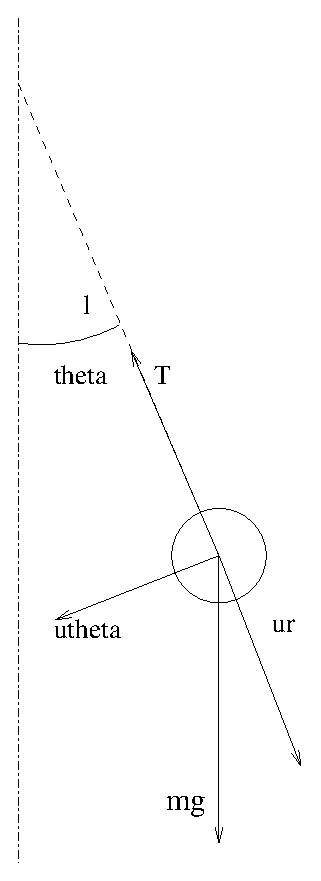
\includegraphics[scale=0.4]{immagini/fisica1/pendolo_forza}
\caption{\index{pendolo}Pendolo semplice.}
\end{figure}
\[\ve F=m\ve g+\ve T=m\ve a\]
\[\left\{
  \begin{array}{l}
  a_r=-\frac{v^2}{l}=-\omega^2 l\\
  a_\theta=\frac{\ud v}{\ud t}
  \end{array}
  \right.\]
\[\left\{
  \begin{array}{l}
  mg\cos\theta-T=-m\omega^2l=-m\frac{v^2}{l}\\
  mg\sin\theta=\frac{\ud v}{\ud t}m
  \end{array}
  \right.\]
\[\omega=\frac{v}{l}=\frac{\ud\theta}{\ud t}\]
\[|v|=\omega l=l\frac{\ud\theta}{\ud t}\]
\[v=-l\frac{\ud\theta}{\ud t}\]
\[mg\sin\theta=-ml\frac{\ud^2\theta}{\ud t}\]
\[g\sin\theta=-l\frac{\ud^2\theta}{\ud t}\]
per piccole oscillazioni\footnote{è il primo sviluppo del polinomio di Taylor}: $\sin\theta\simeq\theta$
\[\frac{\ud^2\theta}{\ud t^2}=-\frac{g}{l}\theta\]
si noti che questa equazione altro non è che l'equazione di un oscillatore armonico\footnote{Questo succede sempre quando si considerano piccole oscillazioni nell'intorno di un punto di equilibrio stabile $x_0$:
\[
 m\ddot x \simeq \underbrace{F(x_0)}_0 + \left.\frac{\ud F}{\ud x}\right|_{x_0} (x-x_0) = k (x-x_0)
\]
con $\left.\frac{\ud F}{\ud x}\right|_{x_0}=k<0$ perché è un punto di equilibrio stabile.
}.
\[g\theta=-l\ddot\theta\qquad \theta=A\sin\left(\omega
t+\varphi\right)\]
\[\theta=-\frac{l}{g}\,\ddot\theta\qquad\ddot\theta=-A\omega^2\sin\left(\omega
t+\varphi\right)=-\omega^2\theta\]
\[\theta=-\frac{\ddot\theta}{\omega^2}\qquad \frac{1}{\omega^2}=\frac{l}{g}\qquad\omega^2=\frac{g}{l}\qquad\omega=\sqrt\frac{g}{l}\]
\[\theta=A\sin\left(\sqrt\frac{g}{l}\,t+\varphi\right)\]
\[2\pi+\sqrt\frac{g}{l}t+\varphi=\sqrt\frac{g}{l}(t+T)+\varphi\qquad
\sqrt\frac{g}{l}T=2\pi\qquad
T=2\pi\sqrt\frac{l}{g}=\frac{2\pi}{\omega}\]

\subsection{\index{forza!variabile!nella velocità}Forze variabili nella velocità}
Su un corpo in caduta agisce la forza di Stokes: $F_s=-\beta v$,
proporzionale alla velocità. $\beta$ dipende dalla viscosità del
mezzo e dalla geometria del corpo.

\[\ve F=m\ve g+\ve F_s=m\ve a\]
\[mg-F_s=ma\]
\[mg-\beta v=ma=m\frac{\ud v}{\ud t}\]
\[mg-\beta v=m\frac{\ud v}{\ud t}\qquad \ud t\left(mg-\beta v\right)=m\ud v\]
\[\int_0^t\ud t=\int_{v_0}^v\frac{m}{mg-\beta v}\,\ud v\]
\[t=\left[-\frac{m}{\beta}\ln\left(mg-\beta
v\right)\right]_{v_0}^{v}=-\frac{m}{\beta}\left(\ln\left(mg-\beta
v\right)-\ln\left(mg-\beta v_0\right)\right)=\]
\[=-\frac{m}{\beta}\ln\frac{mg-\beta v}{mg-\beta v_0}\qquad-\frac{\beta t}{m}=\ln\frac{mg-\beta v}{mg-\beta v_0}\]
\[e^{-\frac{\beta t}{m}}=e^{\ln\frac{mg-\beta v}{mg-\beta v_0}}=\frac{mg-\beta v}{mg-\beta v_0}\]
\[(mg-\beta v)=(mg-\beta v_0)e^{-\frac{\beta t}{m}}\]
\[v=\frac{mg}{\beta}\left(1-e^{-\frac{\beta
t}{m}}\right)+v_0e^{-\frac{\beta t}{m}}\]

se $t\rightarrow +\infty$ allora $v\rightarrow\frac{mg}{\beta}$

se $\beta\rightarrow 0$ allora $v\rightarrow gt+v_0$
\begin{figure}[htbp]
\centering
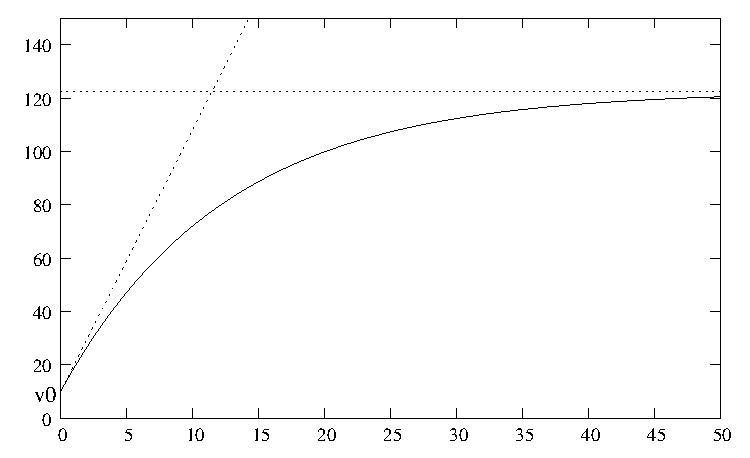
\includegraphics[scale=1]{immagini/fisica1/grafico_forze_nella_velocita}
\caption{Grafico forza variabile nella velocità.}
\end{figure}

\section{\index{forza!apparente}Forze apparenti}
Le forze apparenti non sono delle vere forze, sono degli strumenti che consentono di usare la seconda legge delle dinamica anche in sistemi non inerziali. In particolare le forze apparenti non rispettano il terzo principio della dinamica. Siano $O$ e $O'$ due sistemi di riferimento; $O'$ si muova verso destra con accelerazione $\ve a_{O'}$ rispetto ad $O$. $\ve r_{O'}$ il vettore che individua $O'$ rispetto \mbox{ad $O$.}
\begin{figure}[htbp]
   \centering
   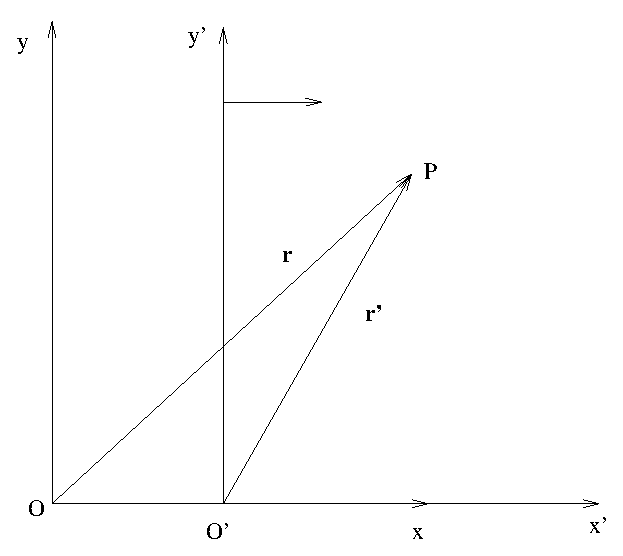
\includegraphics[scale=0.5]{immagini/fisica1/apparenti}
\end{figure}
\[\ve r={\ve r}\,^\prime+\ve r_{O'}\qquad\ve v=\ve v\,'+\ve v_{O'}\qquad\ve a=\ve a\,'+\ve a_{O'}\]
\[m\ve a=m\ve a'+m\ve a_{O'}=\ve F\]
\[m\ve a'=\ve F-m\ve a_{O'}=\ve F+\ve F_\text{app}\]
\[\ve F_\text{app}=-m\ve a_{O'}\]
\subsection{Terra}
La Terra non è un sistema inerziale\index{sistema!inerziale}, infatti ruota intorno al Sole e ruota attorno al proprio asse. Consideriamo quest'ultimo moto:
\begin{figure}[htbp]
   \centering
   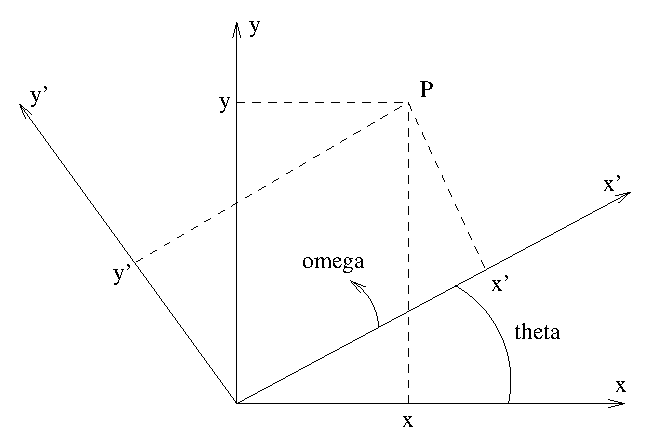
\includegraphics[scale=0.7]{immagini/fisica1/apparenti2}
\end{figure}
\[\left\{\begin{array}{l}
x=x'\cos\theta-y'\sin\theta\\
y=y'\cos\theta+x'\sin\theta
\end{array}\right.\]

\[\left\{\begin{array}{l}
x(t)=x'(t)\cos(\omega t)-y'(t)\sin(\omega t)\\
y(t)=y'(t)\cos(\omega t)+x'(t)\sin(\omega t)
\end{array}\right.\]

\[v_x=\frac{\ud x}{\ud t}=v'_{x'}\cos\left(\omega t\right)-\omega x'\sin\left(\omega t\right)-v'_{y'}\sin\left(\omega t\right)-\omega y'\cos\left(\omega t\right)\]
\begin{align*}
a_x=&\frac{\ud v_x}{\ud t}=a'_{x'}\cos\left(\omega t\right)-\omega v'_{x'}\sin\left(\omega t\right)-\omega v'_{x'}\sin\left(\omega t\right)-\omega^2 x'\cos\left(\omega t\right)-\\
&-a'_{y'}\sin\left(\omega t\right)-\omega v'_{y'}\cos\left(\omega t\right)-\omega v'_{y'}\cos\left(\omega t\right)+\omega^2 y'\sin\left(\omega t\right)\\
=&a'_{x'}\cos\left(\omega t\right)-a'_{y'}\sin\left(\omega t\right)-\omega^2\left[x'\cos\left(\omega t\right)-y'\sin\left(\omega t\right)\right]-\\
&-2\omega\left[v'_{x'}\sin\left(\omega t\right)+v'_{y'}\cos\left(\omega t\right)\right]\\
=&a'_{x}-\omega^2 x-2\omega v'_{y}
\end{align*}
\[\ve \omega\times\ve v'=\left|\begin{array}{ccc}
\ve i&\ve j&\ve k\\
0&0&\omega\\
v'_{x'}&v'_{y'}&v'_{z'}\\
\end{array}
\right|
=-\omega v'_{y'}\ve i+\omega v'_{x'}\ve j\]

\[\left\{\begin{array}{l}
a_x=a'_x-\omega^2 x+2\left(\ve \omega\times\ve v'\right)_x\\
a_y=a'_y-\omega^2 y+2\left(\ve \omega\times\ve v'\right)_y\\
\end{array}\right.\]

\[\ve a=\ve a'-\omega^2 \ve r+2\left(\ve\omega\times\ve v'\right)\]
\[m\ve a=m\ve a'-m\omega^2\ve r+2m\left(\ve\omega\times\ve v'\right)=\ve F\]
\[ma'=\ve F+\underbrace{m\omega^2\ve r}_\text{forza centrifuga}-\underbrace{2m\left(\ve\omega\times\ve v'\right)}_\text{forza di Coriolis}\]\index{Coriolis}\index{forza!centrifuga}\index{forza!di Coriolis}
\[\ve F_\text{cent}=m\omega^2 \ve r\qquad \ve F_\text{Cor}=-2m\left(\ve\omega\times\ve v'\right)\]

\begin{Es}[pendolo di Focault\index{Focault}\index{pendolo!di Focault}]
Se mettiamo un pendolo al polo la forza centrifuga sarà nulla perché $r=0$, ma esiste ancora la forza di Coriolis. Sperimentalmente si osserva che il piano di rotazione del pendolo ruota a causa della non inerzialità della Terra.
\end{Es}
\subsection{Trattazione generale}
Consideriamo due sistemi di riferimento in moto rototraslatorio relativo. Siano $\{\ve{e}_i\}_i^3$ e $\{\ve{e}'_i\}_i^3$ i versori dei due sistemi. Ogni vettore di $O$ si scrive come combinazione lineare i cui coefficienti sono le coordinate $\{x_i\}_i^3$:
\[
 \ve{x}=\sum_{i=1}^3 x_i\ve{e}_i
\]
sia $x_0$ il vettore posizione di $O'$ visto da $O$:
\[
 \ve{x_0}=\sum_{i=1}^3 {x_0}_i \ve{e}_i
\]
nella base del sistema $O'$ il punto individuato da $\ve x$ rispetto al sistema $O$ è individuato dal vettore $\ve{x'}$:
\[
 \ve{x'}=\sum_{i=1}^3 x'_i\ve{e'}_i
\]
La relazione che li lega è:
\[
 \ve{x} =  \ve{x_0}+\ve{x'}
\]
\[
 \ve{v}=\frac{\ud}{\ud t}\ve{x}=\frac{\ud}{\ud t}\ve{x_0}+\frac{\ud}{\ud t}\ve{x'}=\ve{v_0}+\sum_{i=1}^3\left(\underbrace{\frac{\ud x'_i}{\ud t}\ve{e}'_i}_{\ve{v'}}+x'_i\frac{\ud \ve{e}'}{\ud t}\right)
\]
A causa della rotazione il versore del sistema primato ruota, ma il suo modulo non cambia. Dopo un tempo $\ud t$ avrà fatto un angolo $\ud\alpha=\omega\ud t$, quindi per la definizione di angolo $\ud\alpha=\norm{\ud\ve{e'_i}}$. In generale vale:
\[
 \frac{\ud\ve{e'_i}}{\ud t}=\ve\omega\times\ve{e'_i}
\]
quindi:
\[
 \ve{v}=\ve{v'}+\ve{v_0}+\ve{\omega}\times\ve{x'}
\]
si noti come $\ve v'\neq \ve{\dot x'}$, infatti:
\[
 \frac{\ud\ve x'}{\ud t} = \ve v-\frac{\ud}{\ud t} \ve x_0 = \ve v'+\ve\omega\times\ve x'
\]
si definisce velocità di trascinamento la velocità misurata da $O$ di un punto fermo rispetto ad $O'$, cioè per cui $\ve v'=0$:
\[
 \ve v_T = \ve{v_0}+\ve{\omega}\times\ve{x'}
\]
la velocità di trascinamento \index{velocità!di trascinamento}è uguale alla differenza di velocità misurate dai due osservatori: $\ve v_T = \ve{v} - \ve{v'}$.

Derivando la velocità\footnote{tralasciamo i simboli di sommatoria come nella notazione di Einstein}:
\begin{align*}
 \ve{a}&=\frac{\ud}{\ud t}\ve{v}=\frac{\ud}{\ud t}\left(\frac{\ud x'_i}{\ud t}\ve{e'_i}\right)+\frac{\ud\ve{v_0}}{\ud t}+\frac{\ud\ve\omega}{\ud t}\times\ve x'+\ve\omega\times\frac{\ud\ve{x'}}{\ud t}\\
&=\frac{\ud^2 x'_i}{\ud t^2}\ve{e'_i}+\frac{\ud x'_i}{\ud t}\frac{\ud\ve{e'_i}}{\ud t}+\ve{a_0}+\frac{\ud\ve\omega}{\ud t}\times\ve x'+\ve\omega\times\left(\ve{v'}+x'_i\frac{\ud\ve{e'_i}}{\ud t}\right)\\
&=\ve{a'}+\ve\omega\times\ve{v'}+\ve{a_0}+\frac{\ud\ve\omega}{\ud t}\times\ve x'+\ve\omega\times\ve{v'}+\ve\omega\times\left(\ve\omega\times\ve{x'}\right)\\
&=\ve{a'}+\ve{a_0}+\frac{\ud\ve\omega}{\ud t}\times\ve x'+2\ve\omega\times\ve{v'}+\ve{\omega}(\ve\omega\cdot\ve{x'})-\ve{x'}(\ve\omega\cdot\ve\omega)\\
&=\ve{a'}+\ve{a_0}+\frac{\ud\ve\omega}{\ud t}\times\ve x'+2\ve\omega\times\ve{v'}-\omega^2\ve{x'}
\end{align*}
dove nel penultimo passaggio si è usato $\ve A\times(\ve B\times \ve C)=\ve{B}(\ve{A}\cdot\ve{C})-\ve{C}(\ve{A}\cdot\ve{B})$. Moltiplicando per $m$ si ottiene:
\begin{equation}
 \label{eq:newton_non_inerziale}
 m\ve{a'}=\ve F-m\ve{a_0}-m\frac{\ud\ve\omega}{\ud t}\times\ve x'+m\omega^2\ve x'-2m\ve\omega\times\ve{v'}
\end{equation}
L'accelerazione di trascinamento è quella di un punto solidale con $O'$ misurata da $O$, quindi per questo punto $\ve v'=0$ e $\ve a'=0$:
\[
 \ve a_T = \ve{a_0}+\frac{\ud\ve\omega}{\ud t}\times\ve x'-\omega^2\ve{x'}
\]
e quindi:
\[
 \ve a = \ve a'+\ve a_T + \underbrace{2\ve\omega\times\ve v'}_{\ve a_c}
\]
dove $\ve a_C$ è l'\index{accelerazione!di Coriolis}accelerazione di Coriolis.
\subsection{Casi particolari}
\subsubsection{Moto uniformemente accelerato}
Se $O'$ si muove di moto uniformemente accelerato allora in questo sistema di riferimento la legge di Newton si scrive come l'equazione \eqref{eq:newton_non_inerziale} considerando $\omega = 0$:
\begin{equation}
 \ve F = m\ve a'-m\ve a_0
\end{equation}
\subsubsection{Moto circolare uniforme}
Per questo caso $\ve a_0=0$ e $\omega$ è costante:
\begin{equation}
 \ve F = m\ve a' + m\omega^2\ve x' - 2m\ve \omega \times\ve v'
\end{equation}
dove il primo termine addizionale è la \index{forza!centrifuga}forza centrifuga, mentre il secondo è la \index{forza!di Coriolis}forza di Coriolis.

\section{\index{quantità di moto}Quantità di moto}
\begin{Def}[quantità di moto di un punto materiale]
\begin{equation}
\ve{p}:=m\ve{v}
\end{equation}
sinonimi di quantità di moto sono: quantità di modo lineare, momento, momento lineare.
\end{Def}
\[\frac{\ud \ve p}{\ud t}=\frac{\ud\left(m\ve v\right)}{\ud t}=m\ve a=\ve F\]
\[\text{Newton disse: }\ve F=\frac{\ud \ve p}{\ud t}\]
\subsection{Sistema di \texorpdfstring{$N$}{N} punti}
\begin{Def}[quantità di moto di un sistema di $N$ punti]
La quantità di moto totale di un sistema di $N$ punti è la somma delle quantità di moto dei singoli punti.
\begin{equation}
 \ve p=\sum_{I=1}^N\ve p_i=\sum_{i=1}^Nm_i\ve v_i
\end{equation}
\end{Def}
\begin{Teo}
 La variazione della quantità di moto è uguale alle forze esterne
\begin{align*}\frac{\ud \ve p}{\ud t}&=\frac{\ud }{\ud t}\sum^N_{i=1}m_i\ve v_i=\sum_{i=1}^{N}\frac{\ud \left(m\ve v_i\right)}{\ud t}=\sum_{i=1}^{N}m_i\frac{\ud \ve v_i}{\ud t}=\sum_{i=1}^{N}m_i\ve a_i=\\
&=\sum^N_{i=1}\stackrel{\text{Est}}{\ve F_i}+\sum^N_{i=1}\stackrel{\text{Int}}{\ve F_i}=\sum^N_{i=1}\stackrel{\text{Est}}{\ve F_i}\end{align*}
Nell'ultimo passaggio abbiamo usato il terzo principio della dinamica. Si conclude che in un sistema isolato, cioè con
$\sum^N_{i=1}\stackrel{\text{Est}}{\ve F_i}=0$ vale la legge di
conservazione della quantità di moto: $\ve
p=\overrightarrow\const$.
\end{Teo}
\begin{Es}[carrellini]
Due carrellini di massa $m$ e $M$ si urtano frontalmente con
velocità iniziali $v$ e $V$.
\[ P_i= P_f=0\qquad P_f=M V+m v=0\]
\[M V=m v\qquad\frac{V}{v}=\frac{m}{M}\]
\end{Es}

\begin{Es}[decadimento]
L'uranio decade in questo modo:
\[\ce{^{238}_{92}U -> ^{234}_{90}Th + ^{4}_{2}\alpha}\]
\[\ve p_f=m_{\ce{Th}}\ve v_{\ce{Th}}+m_\alpha \ve v_\alpha=\ve p_0=0\]
\[
m_{\ce{Th}}v_{\ce{Th}}=m_\alpha v_\alpha\qquad v_\alpha=\SI{2E7}{\metre\per\second}
\]
\[
v_{\ce{Th}}=\frac{m_\alpha v_\alpha}{m_{\ce{Th}}}=\SI{3.4E5}{\metre\per\second}
\]
\end{Es}

\section{\index{centro di massa}Centro di Massa}
\begin{Def}[Centro di massa di $N$ punti]
\begin{equation}\ve r_{CM}=\frac{\sum^N_{i=1}\left(\ve
r_im_i\right)}{\sum^N_{i=1}m_i}=\frac{\sum^N_{i=1}\left(\ve
r_im_i\right)}{M}\end{equation}
\[x_{CM}=\frac{\sum^N_{i=1}\left(x_im_i\right)}{M} \qquad
y_{CM}=\frac{\sum^N_{i=1}\left(y_im_i\right)}{M}\qquad
z_{CM}=\frac{\sum^N_{i=1}\left(z_im_i\right)}{M}\]
\end{Def}
\[\ve v_{CM}=\frac{\ud \ve r_{CM}}{\ud t}=\frac{\sum^N_{i=1}\frac{\ud}{\ud t}\left(m_i\ve r_i\right)}{\sum^N_{i=1}m_i}=\frac{\sum^N_{i=1}\left(m_i\ve v_i\right)}{M}\]
\[M\ve v_{CM}={\sum^N_{i=1}m_i\ve v_i}=\ve p\]
\[\frac{\ud \ve p}{\ud t}=\frac{\ud}{\ud t}M\ve v_{CM}=M\ve a_{CM}=\sum^N_{i=1}\stackrel{\text{Est}}{\ve F_i}\]
\begin{Teo}
\begin{eqimp}{equation}
M\ve V_{CM}=\ve P \qquad M\ve a_{CM}=\sum \stackrel{\text{Est}}{\ve F_i}
\end{eqimp}
Se il sistema è isolato $\sum \stackrel{\text{Est}}{\ve F}=0$
\[M\ve a_{CM}=0 \Rightarrow \ve a_{CM}=0\]
allora il centro di massa si muove di moto rettilineo uniforme.
\end{Teo}

\subsection{Corpo continuo}
\begin{Def}[Centro di massa per un corpo continuo]
\begin{equation}\ve r_{CM}=\frac{\int_V \ve r\,\ud m}{M}\end{equation}
\end{Def}
\begin{Def}[Densità media]
 \begin{equation}\rho =\frac{m}{V}\end{equation}
\end{Def}
\begin{Def}[Densità locale]
 \begin{equation}\rho(x,y,z)=\frac{\ud m}{\ud V}\end{equation}
\end{Def}
\[\ud m=\rho\,\ud V\]
\[M=\int_V \ud m=\int_V\rho \,\ud V\]
\begin{equation}\ve r_{CM}=\frac{\int_V \ve r \ud V\rho}{M}=\frac{\int_V\rho\ve r\,\ud V}{\int_V \rho \,\ud V}\end{equation}
Se la densità è uguale in tutti i punti il centro di massa è solo un fattore geometrico:
\[\ve r_{CM}=\frac{\int_V\ve r\,\ud V}{V}\]

\begin{Es}[semicirconferenza]
\label{es:semicirconferenza}
\begin{figure}[htp]
 \centering
 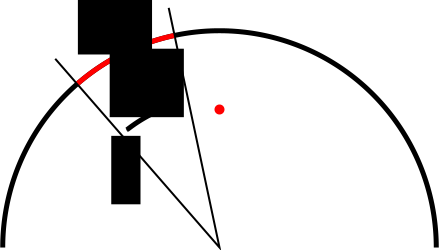
\includegraphics[scale=0.4]{immagini/fisica1/semicerchio}
 \caption{Esempio \ref{es:semicirconferenza}.}
\end{figure}

\[x_{CM}=0 \quad\text{per simmetria}\]
\[\frac{\ud m}{M}=\frac{\ud s}{\pi r}\qquad \ud s=r\ud\theta\]
\[\ud m=\frac{M\ud s}{\pi r}=\frac{Mr\ud\theta}{\pi r}=\frac{M\ud\theta}{\pi}\]
\[y=r \sin \theta\]
\[y_{CM}=\frac{\int y\ud m}{M}=\frac{r}{\pi}\int_0^\pi \sin\theta \ud \theta=-\frac{r}{\pi}\left[\cos\theta\right]_0^\pi=-\frac{r}{\pi}(-1-1)=\frac{2r}{\pi}\]
\end{Es}

\begin{Es}[cerchio bucato]
\label{es:cerchio_bucato}
\begin{figure}[htp]
 \centering
 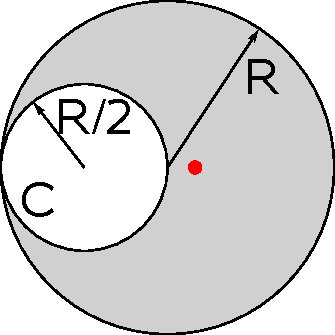
\includegraphics[scale=0.7]{immagini/fisica1/luna}
 \caption{Esempio \ref{es:cerchio_bucato}.}
\end{figure}

Luna è il cerchio grande meno il piccolo ($C$) di raggio
$\frac{r}{2} \quad y_{CM}=0$ per simmetria
\[M^C=\rho\pi\left(\frac{r}{2}\right)^2=\rho\pi\left(r^2-\frac{r^2}{4}\right)=\frac{3}{4}\rho\pi r^2\qquad M^{\text{luna}}=\rho\left(\pi r^2-\pi\left(\frac{r}{2}\right)^2\right)\]
\[x_{CM}^{\text{pieno}}=0=\frac{x_{CM}^{\text{luna}}+x_{CM}^CM^C}{M^C+M^{\text{luna}}}\]
\[0=x_{CM}^{\text{luna}}x_{CM}^C\frac{M^C}{M^{\text{luna}}}=x_{CM}^{\text{luna}}x_{CM}^C\frac{4M^C}{3\rho \pi r^2}=x_{CM}^{\text{luna}}x_{CM}^C\frac{4\rho\pi r^2}{4\cdot 3\rho\pi r^2}=\frac{x_{CM}^{\text{luna}}x_{CM}^C}{3}\]
\[x_{CM}^{\text{luna}}=3x_{CM}^C=\frac{R}{6}\]
\end{Es}

\subsection{\index{teorema!di Pappo--Guldino}Teorema di Pappo--Guldino}
\begin{Teo}[Pappo--Guldino]
Il volume generato dalla rotazione di una superficie è uguale
all'area della superficie per la distanza percorsa dal centro di
massa durante la rotazione.
\end{Teo}
\begin{Es}[Semicerchio]
Il volume generato dalla rotazione del semicerchio è il volume della
sfera: $\frac{4}{3}\pi r^3$, la distanza percorsa dal centro di
massa è $2\pi y$ con $y$ l'ordinata del centro di massa, la
superficie del semicerchio è $\frac{\pi r^2}{2}$, quindi
\[2\pi y\frac{\pi r^2}{2}=\frac{4}{3}\pi r^3\]
\[y=\frac{4}{3\pi}r\]
\end{Es}

\section{\index{impulso di una forza}Impulso di una forza}
\begin{Def}[Impulso di una forza]
L'impulso di una forza $\ve F$ tra il tempo $t_1$ e $t_2$ è definito come:
\begin{equation}
 \ve{J}(t_1,t_2)=\int_{t_1}^{t_2} \ve{F}\, \ud t
\end{equation}
\end{Def}
poiché
\begin{align*}
\int_{t_1}^{t_2} \ve{F}\, \ud t &= \int_{t_1}^{t_2}m\ve a\, \ud t=m\int_{\ve v(t_1)}^{\ve v(t_2)}\frac{d\ve{v}}{\ud t}\,\ud t=m\int_{t_1}^{t_2}\ud \ve{v}\\
&=m\left[\ve v(t_2)-\ve v(t_1)\right]=\ve p_2 - \ve p_1=\Delta \ve p
\end{align*}
allora:
\begin{Teo}[inpulso]
\[
\ve J=\int_{t_1}^{t_2}\ve F \ud t=\Delta \ve p
\]
\end{Teo}
In particolare se il sistema è isolato con due corpi si ha:

\[
\Delta \ve p_1=\int_{t_1}^{t_2} \ve F_{1,2}\, \ud t\qquad \Delta \ve p_2=\int_{t_1}^{t_2} \ve F_{2,1}\, \ud t
\]
\[
\Delta \ve p_1 + \Delta \ve p_2=\int\left(\ve F_{1,2}+\ve F_{2,1}\right)\ud t=0=\Delta\ve p_{\text{totale}}
\]
\[
\ve p_{\text{iniziale}}=\ve p_{\text{finale}}
\]
dove si è usato terzo principio della dinamica. La conservazione della quantità di moto vale in tutti i sistemi isolati.

\section{\index{urti}Urti}
Gli urti si classificano in elastici ed anelastici. Gli urti reali sono una via intermedia. Negli urti elastici si conserva tutta l'energia cinetica, agiscono solo forze conservative; durante l'urto l'energia cinetica si trasforma in energia potenziale, per poi tornare completamente energia cinetica. La quantità di moto si conserva sempre in quanto non agiscono forze esterne.

\subsection{\index{urti!elastici}Urti elastici}

\subsubsection{Urti in 1 dimensione}

\[ \left \{
\begin{array}{ll}
   m_1v_{i,1}+m_2v_{i,2}=m_1v_{f,1}+m_2v_{f,2} & v_{1,f}=? \\
   \frac{1}{2}m_1v_{i,1}^2+\frac{1}{2}m_2v_{i,2}^2=\frac{1}{2}m_1v_{f,1}^2+\frac{1}{2}m_2v_{f,2}^2 & v_{2,f}=?
   \end{array}
   \right.\]
\[v_{1,f}=\frac{2m_2}{m_1+m_2}v_{i,2}-v_{i,1}\frac{m_2-m_1}{m_1+m_2}\]
\[v_{2,f}=\frac{2m_1}{m_1+m_2}v_{i,1}-v_{i,2}\frac{m_1-m_2}{m_1+m_2}\]

\subsubsection{casi limite}
\label{casilimiteurti}
\begin{enumerate}
\item $m_1=m_2$
\[v_{f,1}=v_{i,2}\]
\[v_{f,2}=v_{i,1}\]
  \begin{itemize}
  \item $v_{i,2}=0$
  \[v_{f,1}=0\]
  \[v_{f,2}=v_{i,1}\]
  \end{itemize}
\item $m_2\gg m_1$
\[\frac{m_1}{m_2}\simeq 0\]
\[v_{f,1}=-v_{i,1}+2v_{i,2}\]
\[v_{f,2}=v_{i,2}\]
  \begin{itemize}
  \item $v_{i,2}=0$
  \[v_{f,1}=-v_{i,1}\]
  \[v_{f,2}=v_{i,2}=0\]
  \item $v_{i,1}=0$
  \[v_{f,1}=2v_{i,2}\]
  \[v_{f,2}=v_{i,2}\]
  \end{itemize}

\end{enumerate}

\subsubsection{Urti in due dimensioni}
Due corpi di massa $m_1$, $m_2$, prima dell'urto velocità $\ve v_{i,2}=0$, $\ve v_{i,1}$, il secondo corpo è fermo, dopo l'urto velocità $\ve v_{f,1}$, $\ve v_{f,2}$.

\[\left\{
\begin{array}{l}
m_1\ve v_{i,1}=m_1\ve v_{f,1}+m_2\ve v_{f,2}\\
\frac{1}{2}m_1 v_{i,1}^2=\frac{1}{2}m_1 v_{f,1}^2+\frac{1}{2}m_2
v_{f,2}^2
\end{array}\right.\]

\[\left\{
\begin{array}{l}
m_1v_{i,1}=m_iv_{f,1}\cos\varphi_1+m_2v_{f,2}\cos\varphi_2\\
0=m_1v_{f,1}\sin\varphi_1-m_2v_{f,2}\sin\varphi_2\\
\frac{1}{2}m_1 v_{i,1}^2=\frac{1}{2}m_1 v_{f,1}^2+\frac{1}{2}m_2
v_{f,2}^2
\end{array}\right.\]
Il sistema è formato da 3 equazioni, ma da 4 incognite
($\varphi_1, \varphi_2, v_{f,1}, v_{f,2}$), ha $\infty^1$
soluzioni.

Nel caso particolare di $m_1=m_2$ si ha:
\[\frac{1}{2}m v_{i,1}^2=\frac{1}{2}m
v_{f,1}^2+\frac{1}{2}m v_{f,2}^2\]
\[\left\{
\begin{array}{l}
v_{i,1}^2=v_{f,1}^2+v_{f,2}^2\\
m^2v_{i,1}^2=m^2v_{f,1}^2+m^2v_{f,2}^2+2m^2v_{1,f}v_{2,f}\cos\alpha
\end{array}
\right.\]

\[\left\{
\begin{array}{l}
v_{i,1}^2=v_{f,1}^2+v_{f,2}^2\\
v_{i,1}^2=v_{f,1}^2+v_{f,2}^2+2v_{1,f}v_{2,f}\cos\alpha
\end{array}
\right.\]

quindi $\cos \alpha=0\quad\Rightarrow\quad\alpha=\SI{90}{\degree}$, oppure $v_{1,f}=0$ e $v_{2,f}=v_{1,i}$

\subsection{\index{urti!anelastici}Urti completamente anelastici}

Negli urti anelastici il sistema perde la massima energia cinetica possibile, che non è tutta
in quanto se il sistema perdesse tutta l'energia cinetica violerebbe la conservazione
della quantità di moto. Si dimostra che questo caso è quello in cui dopo l'urto i due corpi
rimangono attaccati.

\begin{Es}[pendolo balistico{\index{pendolo!balistico}}]
Un proiettile di massa $m$, velocità $v$ urta un pendolo balistico di massa $M>m$ e velocità $V=0$. Prima dell'urto la quantità di moto totale del sistema è $mv$, dopo $(M+m)V$.
\[mv=(M+m)V\]
\[V=\frac{mv}{M+v}\]
Dopo l'urto il pendolo balistico, con il proiettile incorporato oscilla come un pendolo, l'energia meccanica si conserva, quindi $K_A=U(B)$


\[\frac{1}{2}(m+M)V^2=(m+M)gh\]
\[\frac{1}{2}\left(\frac{mv}{M+m}\right)^2=(m+M)gh\]
\[\frac{1}{2}\frac{m^2v^2}{M+m}=(m+M)gh\]
\[v^2=\frac{(m+M)gh\cdot 2(m+M)}{m^2}=\frac{2(m+M)^2gh}{m^2}\]
\[v=\frac{m+M}{m}\sqrt{2gh}\]
Consideriamo un sistema di riferimento $\ast$ inerziale rispetto
al CM con la stessa velocità del CM.

\[\ve P^\ast_{\text{prima}}=(m+M)\ve V_{\text{CM}}^\ast=0\]
\[\ve P^\ast_{\text{dopo}}=0\quad\text{sono attaccati}\quad \ve
v=0\] Quindi tutta l'energia cinetica è persa.
\end{Es}
\section{\index{momento!d'inerzia}Momento d'inerzia}
Corpo rigido(CR): presi due punti qualsiasi la loro distanza
rimane inalterata. Servono tre punti, quindi 9 coordinate, ma le
distanze rimangono fisse nel tempo, quindi il corpo ha 6 gradi di
libertà. Per descrivere il moto di un corpo bisogna dare 6
coordinate in funzione del tempo. Se fissiamo un asse di rotazione
si ha un solo grado di libertà. In questo caso si ha una rotazione
intorno ad un asse fisso. Ogni punto del CR descrive una
circonferenza. $\theta$ è comune a tutti, quindi anche $\omega$ e
$\alpha$
\[\ud s_i=\ud \theta r_i\]
\[v_i=r_i\omega \qquad a_t=\frac{\ud v_i}{\ud t}=\alpha r_i\]
\[K=\sum_i\frac{1}{2}m_iv_i^2\]
\[K=\sum_i\frac{1}{2}m_i\omega^2r_i^2=\frac{1}{2}\omega^2\left(\sum_im_ir_i^2\right)=\frac{1}{2}I\omega^2\]
\[I=\text{momento d'inerzia}=\sum_{i=1}^N m_ir_i^2\]
\[\text{Nel caso di corpo continuo} \sum_{i=1}^\infty \ud m_ir_i^2=\int_V  r^2\,\ud m\]
Essendo $\ve r$ relativo a un punto $O$ allora anche $I$ sarà relativo ad $O$. Bisogna sempre specificare rispetto quale punto si calcola $I$.

\subsection{Calcolo Momenti di Inerzia}

\begin{minipage}[c]{\textwidth}
\subsubsection{Barra Sottile per l'estremo}

   \centering
   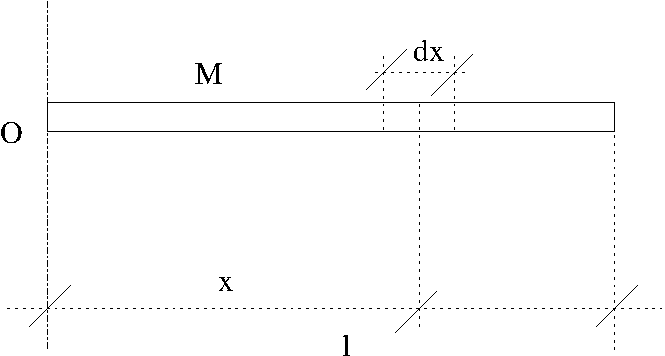
\includegraphics[scale=0.4]{immagini/fisica1/sbarra_sottile1}

\[\frac{\ud m}{M}=\frac{\ud x}{l}\]
\[I_0=\int_0^l\frac{M}{l}\ud x x^2=\frac{M}{l}\left[\frac{x^3}{3}\right]_0^l=\frac{M}{l}\frac{l^3}{3}=\frac{M}{3}l^2\]
\end{minipage}

\subsubsection{Barra sottile per il centro di massa}
\[I_c=\int_{-l/2}^{l/2}\frac{M}{l}\ud x
x^2=\frac{M}{l}\int_{-l/2}^{l/2}x^2 \ud
x=\frac{M}{3l}\left(\frac{l^3}{8}+\frac{l^3}{8}\right)=\frac{M}{12}l^2\]

\subsubsection{Disco}


\begin{figure}[htbp]
   \centering
   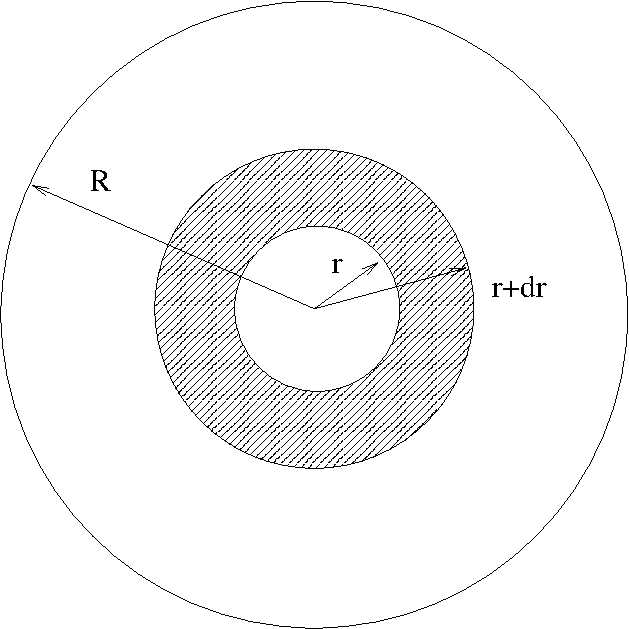
\includegraphics[scale=0.3]{immagini/fisica1/disco}
\end{figure}

\[\frac{\ud m}{M}=\frac{2\pi r\ud r}{\pi R^2}\]
\[\ud m=M\frac{2\ud r}{R^2}r\]
\[I_O=\int_O^R\frac{M}{R^2}2\ud r r^3=\frac{2M}{R^2}\int_O^R r^3
\ud r=\frac{2M}{R^2}\cdot\frac{R^4}{4}=\frac{1}{2}MR^2\]

\subsubsection{Sfera omogenea}

\begin{minipage}[]{\textwidth}
Dividiamo la sfera in tanti dischetti:
\vspace{0.7cm}

   \centering
   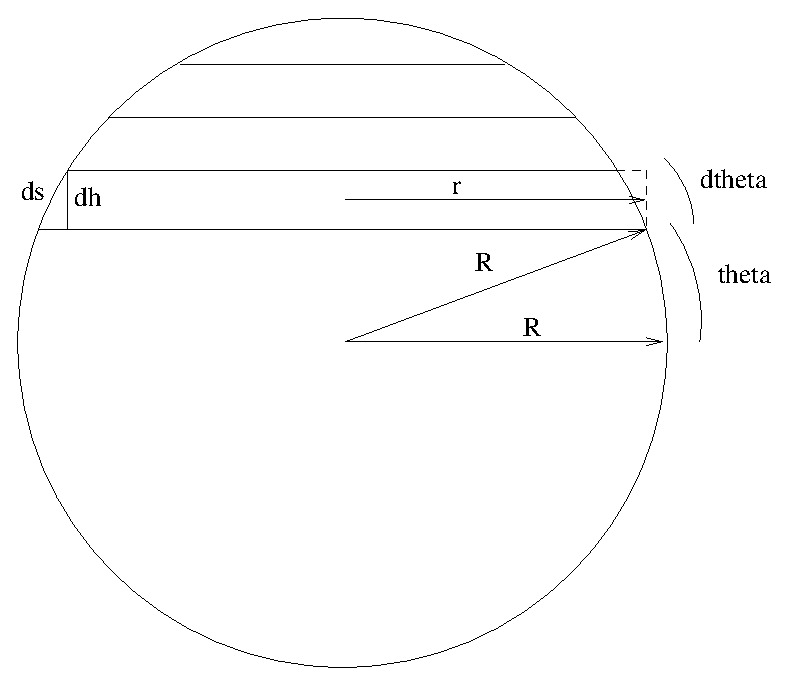
\includegraphics[scale=0.45]{immagini/fisica1/sfera_omogenea1}

\end{minipage}
\[r=R\cos\theta\quad \ud s=R\ud\theta\quad \ud h=\ud s\cos\theta=R\ud\theta\cos\theta\]
\[\ud m=\rho\ud V=\rho\pi r^2\ud h=\rho\pi R^2\cos^2\theta R\cos\theta\ud\theta=R^3\rho\pi\cos^3\theta\ud\theta\]
\[I_\text{dischetto}=\ud I=\frac{1}{2}\ud m r^2=\frac{1}{2}\rho\pi R^3\cos^3\theta\ud\theta R^2\cos^2\theta=\frac{1}{2}\rho\pi R^5\cos^5\theta\ud\theta\]
\[m=\rho\frac{4}{3}\pi R^3\]
\[I_\text{sfera}=2\int_0^\frac{\pi}{2}\ud I=\frac{3}{4}mR^2\int_0^\frac{\pi}{2}\cos^5\theta\ud\theta=\frac{2}{5}mR^2\]

\subsection{\index{teorema!di Steiner}\index{teorema!degli assi paralleli}Teorema di Steiner o degli assi paralleli}
\begin{Teo}[Steiner o degli assi paralleli]Sia $d$ la distanza da un asse di rotazione $I_0$ parallelo all'asse $I_{CM}$ passante per il centro di massa. Allora:
\[I_0=d^2M+I_{CM}\]
\end{Teo}
\begin{figure}[htbp]
   \centering
   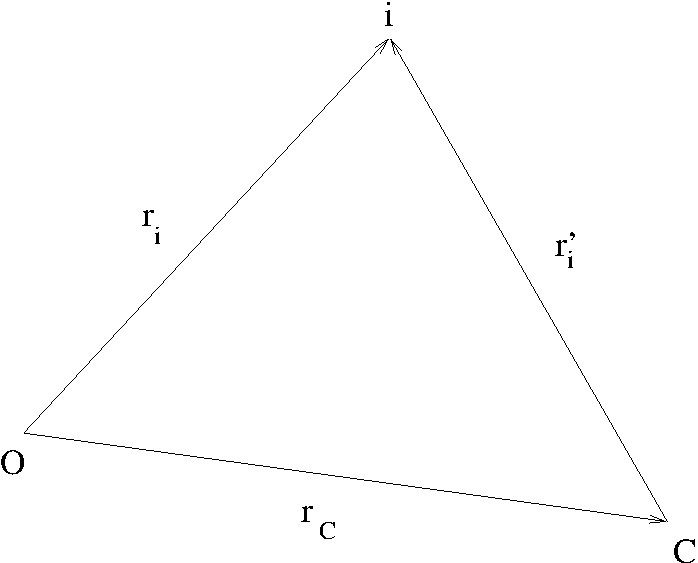
\includegraphics[scale=0.45]{immagini/fisica1/steiner}
\end{figure}
\[\ve r_i=\ve r_C+\ve r_i\,'\]
\[\ve r_i\cdot\ve r_i=r_i^2=\left(\ve
r_C+r_i\,'\right)\cdot\left(\ve r_C+\ve r_i\,'\right)\Rightarrow
r_i^2=r_C^2+r_i\,'^2+2\ve r_C\cdot\ve r_i\,'\]
\begin{align*}
I_0&=\sum m_ir_i^2=\sum r_C^2m_i+\sum r_i\,'^2m_i+\sum m_i
\cdot 2\ve r_C\cdot \ve r_i\,'\\
&=r_C^2\sum m_i+I_C+2\ve
r_C\cdot\sum m_i\ve r_i\,'=d^2M+I_{C}+2\ve r_C\cdot\sum m_i\cdot
\ve r_i\,'\end{align*}
Per ipotesi $C$ è il $CM$ del sistema
\[I_0=d^2 M+I_{CM}+2\ve r_i\frac{\sum m_i\ve r_i\,'}{M}\cdot
M=d^2M+I_{CM}+2\ve r_i\cdot \ve r\,_{CM}^{CM} M=d^2M+I_{CM}\]
Ma $Md^2>0$ quindi $I_{CM}$ è il momento minimo possibile.
\begin{Es}
Il momento d'inerzia di una circonferenza rispetto al centro di massa è \mbox{$I_{CM}=\frac{1}{2}MR^2$}, per un estremo è:
\[I_0=I_{CM}+MR^2=\frac{1}{2}MR^2+MR^2=\frac{3}{2}MR^2>I_{CM}\]
\end{Es}
\section{\index{momento!di una forza}Momento di una forza}
\begin{Def}[Momento di una forza]
Il momento di una forza (o momento torcente) rispetto ad un polo fisso $O$
 \begin{equation}
  \ve{\tau}_O=\ve r \times \ve F
 \end{equation}
dove $\ve r$ è il vettore che individua il punto di applicazione dela forza rispetto al polo.
\end{Def}
\[\delta L=\ud K\qquad \ud \ve s=\ve r\ud \theta\]
\[\delta L=F\ud s\cos \phi=Fr\ud\theta\cos\phi\]
\[K=\frac{1}{2}I\omega^2\qquad\ud K=I\omega\ud\omega\]
\[Fr\ud\theta\cos\phi=I\omega\ud\omega\]
\[Fr\frac{\ud\theta}{\ud t}\cos\phi=I\omega\frac{\ud\omega}{\ud
t}\]
\[Fr\omega\cos\phi=I\omega\alpha\]
\[Fr\cos\phi=I\alpha\]
\[Fr\sin\beta=I\alpha\]
\[\ve\tau=I\ve\alpha\qquad\text{analoga a $\ve F=m\ve a$}\]
\section[\index{momento!angolare}\index{momento!della quantità di moto}Momento angolare o della quantità di moto]{Momento angolare\\ o momento della quantità di moto}
\[\ve l_0=\ve r\times m\ve v\qquad\text{rispetto al polo $0$ fisso.}\]
\begin{align*}
\frac{\ud \ve l_0}{\ud t}&=\frac{\ud}{\ud t}\left(\ve r\times m\ve v\right)= \frac{\ud\ve r}{\ud t}\times m\ve v+\ve r\times\frac{\ud m\ve v}{\ud t}\\
&=\ve v\times m\ve v+\ve r \times m\ve a=\ve r\times m\ve a=\ve r\times\ve F=\ve \tau_0
\end{align*}
\[\frac{\ud\ve l_0}{\ud t}=\ve \tau_0\qquad\text{analoga
a}\qquad\frac{\ud \ve p}{\ud t}=\ve F\]
\subsection{Sistema di N punti}
\[\ve L_0=\sum_{i=1}^N \ve l_{0_i}\]
\begin{align*}\frac{\ud \ve L_0}{\ud t}&=\sum_{i=1}^{N}\frac{\ud \ve l_{0_i}}{\ud
t}=\sum_{i=1}^{N}\frac{\ud}{\ud t}\left(\ve r_i \times \ve
v_i\right)=\sum_{i=1}^{N}\ve v_i\times m_i \ve v_i+\ve
r_i\times m_i\ve a_i\\
&=\sum_{i=1}^{N}\ve r_i\times m_i\ve
a_i=\sum_{i=1}^{N}\ve r_i\times\ve F_i\\
&=\sum_{i=1}^{N}\ve
r_i\times\stackrel{\text{Int}}{\ve F_i}+\sum_{i=1}^{N}\ve
r_i\times\stackrel{\text{Est}}{\ve F_i}=\sum_{i=1}^{N}\ve
r_i\times \stackrel{\text{Est}}{\ve
F_i}=\sum_{i=1}^{N}\stackrel{\text{Est}}{\ve \tau_0}\end{align*}
\subsubsection{Dimostrazione $\stackrel{\text{Int}}{\ve\tau_0}=0$}
\[\ve F_{1,2}=-\ve F_{2,1}\]
\[\ve r_1\times \ve F_{1,2}+\ve r_2\times\ve F_{2,1}=\ve r_1\times \ve F_{1,2}-\ve r_2\times\ve F_{1,2}=\left(\ve r_i-\ve r_2\right)\times\ve F_{1,2}=0\]
perché $\left(\ve r_1-\ve r_2\right)\parallel \ve F_{1,2}$
\subsection{Conservazione del momento angolare}
Se il sistema è isolato si ha: $\stackrel{\text{Est}}{\ve
F}=0\Rightarrow \stackrel{\text{Est}}{\ve \tau}=0$
\[\frac{\ud \ve L_0}{\ud t}=\ve \tau_0=0\qquad \ve
L_0=\overrightarrow{\const}\]
 e quindi
$I\omega={\const}$. Tutto ciò per la simmetria per
rotazioni.
\subsection{Rotazione intorno a \texorpdfstring{$O'$}{O'} mobile}
\[\ve r_i=\ve r_{O'}+\ve r_i\,'\qquad \ve r_i\,'=\ve r_i-\ve r_{O'}\]
\[L_{O'}=\sum\ve r_i\,'\times m\ve v_i=\sum(\ve r_i-\ve
r_{O'})\times m\ve v_i\]
\begin{align*}
\frac{\ud L_{O'}}{\ud t}&=\sum(v_i-v_{O'})\times m\ve v_i+r_i\,' m\ve a_i=-\sum\ve v_{O'}\times m_i\ve v_i+\sum\ve r_i\,'\times\ve F_i\\
&=\ve v_{O'}\times\sum m_i\ve v_i+\ve \tau_{O'}=-\ve
v_{O'}\times\ve P+\stackrel{\text{Est}}{\tau_{O'}}
\end{align*}
\[\frac{\ud L_O}{\ud t}=-\ve v_{O'}\times\ve P+\stackrel{\text{Est}}{\tau_{O'}}\]

se $v_{O'}=0$ allora $-v_{O'}\times\ve P=0$

se $O'=CM$ allora $M\ve V_{CM}=\ve p\Rightarrow\ve
v_{CM}\parallel\ve P\Rightarrow -\ve v_O\times\ve P=0$

\subsection{Rotazione intorno ad un asse}
\[\ve l_i=\ve r_i\times m_i\ve v_i\]
\[l_{i_z}=|\ve l_i|\sin\theta_i\]
\[|\ve l_i|=r_im_iv_i\qquad l_{i_z}=r_im_iv_i\sin\theta_i\qquad
\omega d_i=v_i\]
\[l_{i_z}=m_id_i\omega d_i=md_i^2\omega\]
\[l_{i_z}=m_i\omega R_i^2\]
\[L_z=\sum l_{i_z}=\sum(m_id_i^2)\omega=I\omega\]
\[L_z=I\omega\]
\[\frac{\ud l_{i_z}}{\ud t}=I\frac{\ud \omega}{\ud
t}=I\alpha\qquad \stackrel{\text{Est}}{\tau_{z}}=I\alpha\]
\subsection{Corpo simmetrico rispetto all'asse di rotazione}
\[\ve l_i+\ve l_{i'}=\alpha\ve k\]
\[L=I\omega=L_z\]


\section{Analogia tra grandezze lineari e \mbox{rotazionali}}
\begin{small}
\begin{tabular}{p{4.0cm}p{2.45cm}p{4.0cm}p{2.38cm}}
\hline
Grandezze lineari &&Grandezze rotazionali&\\
\hline
velocità&$\ve v=\ud \ve r/\ud t$ & velocità angolare&$\ve\omega=\ud \phi/\ud t$\\
Accelerazione&$\ve a=\ud \ve v/\ud t$&Accelerazione
angolare&$\ve\alpha=\ud \ve\omega/\ud t$\\
Massa&$m$&Momento d'inerzia&$I=\sum mr^2$\\
Forza&$\ve F$&Momento di una forza&$\ve \tau=\ve r\times \ve F$\\
Seconda legge di Newton&$\sum \stackrel{\text{Est}}{\ve F}=m\ve
a$& Seconda legge di Newton per moto rotatori con asse
fisso&$\sum\stackrel{\text{Est}}{\ve \tau_z}=I\alpha_z$\\
Condizione di equilibrio&$\sum\stackrel{\text{Est}}{\ve
F}=0$&Condizione di equilibrio&$\sum\stackrel{\text{Est}}{\ve
\tau}=0$\\
quantità di moto di una particella&$\ve p=m\ve v$&Momento
angolare di una particella&$\ve l=\ve r\times \ve p$\\
quantità di moto di un sistema di particelle&$\ve P=M\ve
v_{CM}$&Momento angolare di un sistema di particelle&$\ve
L=I\omega$\\
Forma generale della seconda legge di
Newton&$\sum\stackrel{\text{Est}}{\ve F}=\ud \ve P/\ud t$&Forma
generale della seconda legge di Newton per i moti
rotatori&$\sum\stackrel{\text{Est}}{\ve \tau}=\ud \ve L/\ud t$\\
Conservazione della quantità di moto di un sistema di particelle
per il quale $\sum\stackrel{\text{Est}}{\ve F}=0$&$\ve P=\sum
\ve p_n=$ \mbox{$=\overrightarrow\const$}&Conservazione del momento angolare di un sistema di particelle per il quale $\sum\stackrel{\text{Est}}{\ve \tau}=0$&$\ve L=\sum \ve l_n=$ \mbox{$=\overrightarrow\const$}\\
\hline
\end{tabular}
\end{small}

\chapter{Lavoro ed energia}
\minitoc
\section{\index{lavoro}Lavoro definizione}
\begin{Def}[lavoro]
Definiamo lavoro $L$ fatto dalla forza $\ve F$ sul punto $P$ di applicazione della forza lungo il percorso $\Gamma$ l'integrale su $\Gamma$ della forma differenziale $\delta L = \ve F\cdot\ud\ve s$:
\begin{equation}
L=\int_\Gamma\ve F\cdot\ud \ve s
\end{equation}
Il lavoro è una grandezza scalare. Nel SI si misura in joule ($\joule$)\index{Joule}.
\end{Def}
Distinguiamo i seguenti casi particolari:
\begin{description}
\item[Forza parallela]
\[\ve F \parallel \ud\ve s\Rightarrow L=\int_\Gamma F(\ve r)\,\ud s\]
\item[Forza costante]
\[\ve F = \overrightarrow\const\Rightarrow L=\ve F \cdot \ve s = Fs\cos\alpha\]
\item[Forza costante e parallela allo spostamento]
\[\ve F = \overrightarrow\const, \ve F \parallel \ud\ve s\Rightarrow L=Fs\]
\end{description}
\begin{Es}[Forza peso e piano inclinato]
 In questo caso la forza peso sul punto di applicazione è costante $\ve F=m\ve g$, lo spostamento $s$ però non è parallelo, ma forma con la forza peso $\pi/2 -\alpha$ dove $\alpha$ è l'angolo del piano inclinato.
\[
 L = m\ve g \cdot \ve s = mgs\cos(\pi/2 - \alpha) = mgs\sin\alpha = mgh
\]
dove $s$ è la lunghezza del piano inclinato e h la sua altezza.
\end{Es}

\begin{Es}[attrito costante su traiettoria semicircolare orizzontale]
\[F_A=\mu N=\mu mg\quad \delta L=\ve F_A\cdot\ud \ve s=-\mu mg\ud s\]
\[L=\int_\Gamma \delta L=\int_\Gamma -\mu mg\,\ud s=-\mu mg\int_\Gamma\ud
s=-\mu mg\pi R\]
\end{Es}
\subsection{Lavoro nei moti rotatori}
Consideriamo un corpo rigido ruotante attorno ad un asse. Sia $\ud s$ lo spostamento
infinitesimo corrispondete a $\ud \theta$, $\phi$ l'angolo
compreso tra la forza e il vettore $\ve r$:
\[
\delta L=\ve F\cdot\ud\ve s=(F\sin \phi)\ud s=(F \sin \phi)(r
\ud\theta)=(rF\sin\phi)\ud \theta=\tau_z\ud\theta
\]
\[L=\int_{\theta_i}^{\theta_f}\tau_z\ud\theta\]
Se durante la rotazione il momento torcente resta costante, il
lavoro svolto da questo momento torcente è:
\[L=\tau_z\theta\]
\section{\index{potenza}Potenza}
\begin{Def}[potenza]
\begin{equation}
 P=\frac{\ud L}{\ud t}
\end{equation}
\end{Def}
La potenza si misura nel SI in $\joule\per\second$ cioè \watt(watt\index{watt}).
\begin{equation}
P=\frac{\ud L}{\ud t}=\frac{\ve F\cdot\ud \ve s}{\ud t}=\ve F\cdot\frac{\ud \ve s}{\ud
t}=\ve F\cdot \ve v
\end{equation}

\subsection{Potenza nei moti rotatori}
\begin{equation}
P=\frac{\ud L}{\ud t}=\frac{\tau_z\ud\theta}{\ud
t}=\tau_z\omega
\end{equation}

\section[Energia Cinetica]{\index{energia!cinetica}Energia Cinetica}
\begin{Def}[energia cinetica]
\[K=\frac{1}{2}mv^2\]
\end{Def}
A volte indicata con $T$.
\subsection{Teorema lavoro--energia\index{teorema!lavoro--energia}}
\[\delta L=\ve F\cdot\ud \ve s=\ve F\cdot\frac{\ud \ve s}{\ud t}\ud t=\ve F\cdot\ve v\ud t=m\ve a\cdot\ve v\ud t=m\frac{\ud \ve v}{\ud t}\cdot\ve v\ud t=m\ve v\ud \ve v=mv\ud v\]
\[\ud K=\ud \left(\frac{1}{2}mv^2\right)=\ud \left(\frac{1}{2}mvv\right)=\frac{1}{2}m\left(\ud vv+v\ud v\right)=\frac{1}{2}m2v\ud v=mv\ud v\]
\[\delta L=\ud K\qquad\int_A^B\delta L=\int_A^B \ud K\]
\begin{Teo}[lavoro--energia]
\[L=K_B-K_A=\Delta K\]
\end{Teo}
Il lavoro è allora la variazione dell'energia cinetica


\section{Complementi -- Funzioni in due variabili}

\[z=f(x,y)\]
\index{derivata!parziale}derivata parziale:
\[\frac{\partial z}{\partial x}=\frac{\partial f}{\partial x}=\frac{\ud f}{\ud x}\ \text{considerando $y$ costante}\]
derivate seconde parziali:
\[
\frac{\partial^2 z}{\partial x^2}\qquad \frac{\partial^2
z}{\partial y^2}\qquad \frac{\partial^2 z}{\partial x\partial
y}\qquad\frac{\partial^2 z}{\partial y\partial x}\]
\begin{Teo}[Shwartz]
Sotto opportune ipotesi\footnote{Sia $\Omega\subseteq\field{R}^n$ aperto e sia $f:\Omega\to\mathbb{R}$. Supponiamo che le derivate parziali miste $\frac{\partial^2 f}{\partial x_k\partial x_j}$, $\frac{\partial^2 f}{\partial x_j\partial x_k}$ esistano in un intorno di $a\in\Omega$ e siano continue in $a$. Allora esse sono uguali in $a$} le derivate seconde parziali incrociate sono uguali:
\[\frac{\partial^2 z}{\partial x\partial y}=\frac{\partial^2 z}{\partial y\partial x}\]
\end{Teo}
\begin{Def}[\index{forma differenziale! lineare}Forma differenziale lineare]
\[\delta G=H(x,y)\ud x+K(x,y)\ud y\]
\end{Def}
\begin{Def}[\index{differenziale!totale}\index{differenziale!esatto}Differenziale totale o esatto]
\[\ud z=\frac{\partial z}{\partial x}\,\ud x+\frac{\partial z}{\partial y}\,\ud y\]
\end{Def}
è una forma differenziale lineare.
\begin{Teo}
 Una forma differenziale lineare è un differenziale esatto se e
solo se:
\[\frac{\partial H}{\partial y}=\frac{\partial K}{\partial x}\]
\end{Teo}
Il lavoro elementare è una forma differenziale lineare:
\[\delta L=\ve F\cdot \ud \ve s=F_x\ud x+F_y\ud y=F_x(x,y)\ud x+F_y(x,y)\ud y\]
\[L_A^B=\int_A^B\delta L=\int_A^B F_x(x,y)\ud x+F_y(x,y)\ud y\]
\[\text{se } \frac{\partial F_x}{\partial y}=\frac{\partial F_y}{\partial x} \Rightarrow \delta L= \text{differenziale totale}\]
\[\delta L=\ud L=\ud V\]
Allora si avrà, qualunque sia il cammino percorso:
\[L_A^B=\int_A^B \ud V=V(B)-V(A)\]
e la \index{forza!conservativa}forza si dice conservativa.
\[F_x(x,y)=\frac{\partial V}{\partial x}\qquad F_y(x,y)=\frac{\partial V}{\partial y}\]
In termini sintetici:
 \[\ve F=\ve\nabla V\]
 Per dettagli sull'operatore
gradiente vedi sezione \ref{gradiente} a pagina
\pageref{gradiente}.

\subsection{\index{circuitazione!di una forza}Circuitazione di una forza}
\`E il lavoro calcolato su una traiettoria chiusa
\[\oint \ve F\cdot\ud \ve s=0 \quad \text{se la forza è conservativa}\]

\section{\index{energia!potenziale}Energia Potenziale}
\[U=-V\]
\[L_A^B=U(A)-U(B)=-\Delta U\]
Considerando l'energia potenziale in $0$ nulla si ha\footnote{c'è molta confusione sulle notazioni, frequentemente quello che qui è chiamato $V$ è chiamato $U$ e l'energia potenziale $U$ è chiamata $V$}:
\[L_0^P=U(0)-U(P)=0-U(P)\]
\[U(P)=-L_0^P=-\int_0^P \ve{F}\cdot\ud \ve{s}\]
\[\ve F=-\ve\nabla U\]

\subsection{\index{conservazione! dell'energia meccanica}Conservazione dell'energia meccanica}
\begin{Def}[Energia meccanica]
 L'energia meccanica è la somma di energia cinetica e energia potenziale.
\end{Def}
\begin{Teo}[Conservazione energia meccanica]
Considerando solo forze conservative:
\[L_A^B=U_A-U_B\qquad L_A^B=K_B-K_A\]
\[U_A+K_A=U_B+K_B\]
\[U(P)+K=E=\const\]
\end{Teo}
\index{forza!conservativa}Per verificare se una forza è conservativa:

\begin{enumerate}
\item
\[\frac {\partial F_x}{\partial y}=\frac {\partial
F_y}{\partial x}
\]
 se sì allora è conservativa, se no non lo è

\item\[U(0)=0 \qquad L_0^P=U(0)-U(P)=-U(P)\]
\[U(P)=-\int_0^P \ve F\cdot\ud \ve s\]

\item Verifica
\[\frac {\partial U}{\partial x}=-F_x \qquad \frac{\partial U}{\partial y}=-F_y\]
\end{enumerate}
\begin{Es}[Forza peso $F_x=0 \quad F_y=mg$]
\begin{enumerate}
\item $\frac {\partial F_x}{\partial y}=0=\frac {\partial
F_y}{\partial x}$

\item $U(P)=-\int_0^P  \ve F\, \ud \ve s=\int_0^P F_x\, \ud x+F_y\, \ud
y=\int_0^P mg \, \ud y = mgy$

\item $\frac {\partial U}{\partial x}=0=-F_x\quad \frac {\partial
U}{\partial y}=mg=-F_y$
\end{enumerate}
\end{Es}
\begin{Es}[Forza elastica $F_x=-kx \quad F_y=-ky$]
\begin{enumerate}
\item$\frac {\partial F_x}{\partial y}=0=\frac {\partial
F_y}{\partial x}$

\item$U(P)=-\int_0^P \ve F\, \ud \ve s=\left(\int_0^P F_x\, \ud x+\int_0^P
F_y\, \ud y \right)=\frac
{1}{2}kx^2+\frac{1}{2}ky^2=\frac{1}{2}kr^2$

\item$\frac{\partial U}{\partial x}=kx=-F_x \quad \frac{\partial
U}{\partial y}=ky=-F_y$
\end{enumerate}
\end{Es}
\begin{Es}[Forza gravitazionale $ \ve{F}=-G\frac{Mm}{{r^3}}\ve r \quad
r=\sqrt{x^2+y^2}$]

\begin{enumerate}

\item
\[F_x=\frac {-GMm}{r^3}x=-GMmx(x^2+y^2)^{-\frac{3}{2}}\]
\[F_y=\frac {-GMm}{r^3}y=-GMmy(x^2+y^2)^{-\frac{3}{2}}\]
\[\frac{\partial F_x}{\partial y}=GmMx\frac {3}{2}(x^2+y^2)^{-\frac{5}{2}}2y=\frac{\partial F_y}{\partial x}=GmMy\frac {3}{2}(x^2+y^2)^{-\frac{5}{2}}2x \]
\[\frac{\partial F_x}{\partial y}=\frac{\partial F_y}{\partial x}\quad \Rightarrow\quad \text{è conservativa}\]

\item\[U(\infty)=0\]
  \[U(P)=-\int_\infty ^P \ve F \ud \ve s=\int_P^\infty \ve F\ud \ve s=\int_P^\infty -\frac{GMm}{r^2}\ud r=\left[\frac{GMm}{r}\right]_r^\infty=-\frac{GMm}{r}\]
\end{enumerate}
\end{Es}
\subsubsection{Calcolo della \index{velocità!di fuga}velocità di fuga}

conservazione dell'energia: $E_A=E_B$
\[\frac{1}{2}mv_0^2+\left(\frac{-GMm}{r}\right)=\frac{1}{2}mv_\infty^2+0\geq0\]
Caso limite all'$\infty$ arriva fermo $v_\infty=0$
\[\frac{1}{2}mv_0^2-\frac{GMm}{r}=0\]
\[v_0=\sqrt{\frac{2GM}{R}}=\sqrt{2Rg}\simeq \SI{11E3}{\meter\per\second} \quad \text{dalla Terra}\]


\subsubsection{Applicazione dell'energia a \index{pendolo}pendoli}
\begin{figure}[htbp]
\centering
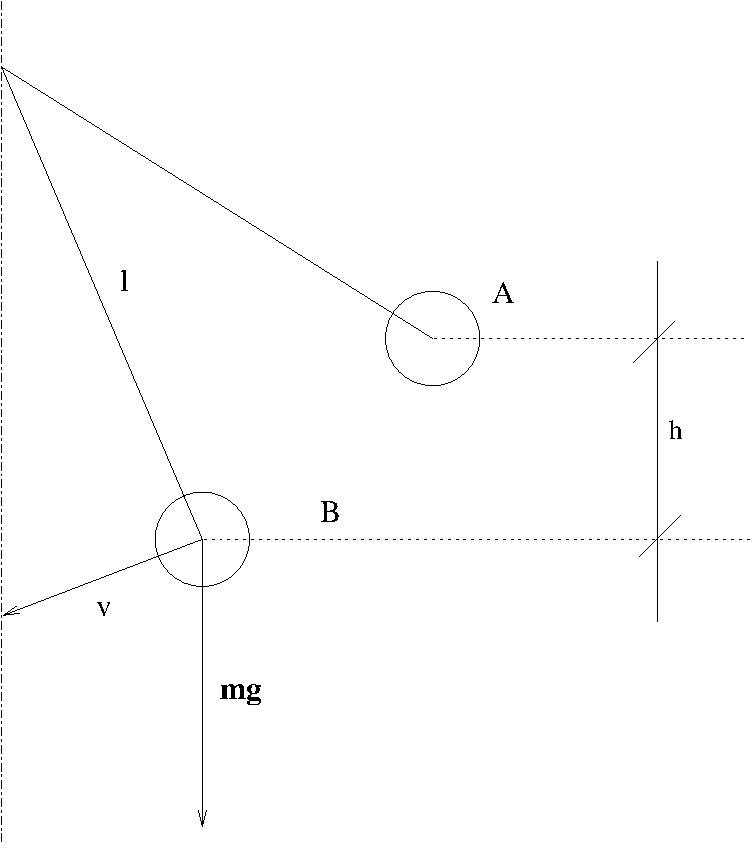
\includegraphics[scale=0.4]{immagini/fisica1/Pendolo_energia}
\end{figure}
Angoli non piccoli, $\ve T\bot \ve v \qquad \ve T\bot \ud\ve s$
\[\delta L=\ve T \cdotp \ud\ve s=0\]
\[U=mgh \qquad K=\frac{1}{2}mv^2\]
\[mgh+\frac{1}{2}mv^2=E=\const\]
A $\theta_0$ si trova nella posizione $A\quad K_A=0$
\[E_A=0+mgh\]
In $B$ $K_B\neq 0\quad E_B=K+mgh_B$
\[h=l-l\cos\theta\]
\[E_A=mg\left(l-l\cos\theta_0\right)\]
\[E_B=\frac{1}{2}mv^2+mg\left(l-l\cos\theta\right)\]
\[E_A=E_B\]
\[mgl\left(1-\cos\theta_0\right)=\frac{1}{2}mv^2+mgl\left(1-\cos\theta\right)\]
\[v^2=2gl(\cos\theta-\cos\theta_0)\]

\begin{Es}[arriva in alto?]
\begin{figure}[htbp]
\centering
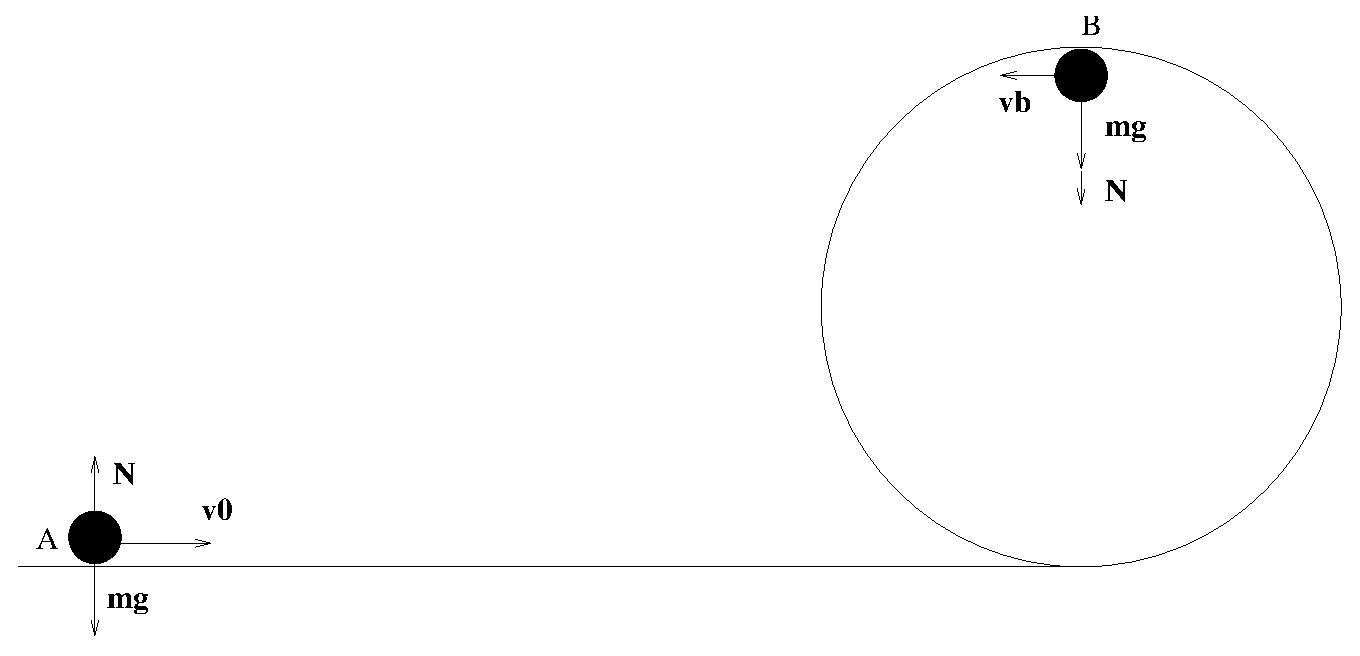
\includegraphics[scale=0.4]{immagini/fisica1/arriva_in_alto}
\end{figure}
La $\ve N$ non compie lavoro perché $\ve N\bot \ud\ve s$
\[E_A=\frac{1}{2}mv_0^2 \qquad E_B=\frac{1}{2}mv_B^2+mg2R\]
\[E_A=E_B \quad E_A=\frac{1}{2}mv_0^2=\frac{1}{2}mv_B^2+mg2R\]
\[v_0^2=v_B^2+4gR\]
Quando è in B
\[mg+N=m\frac{v_B^2}{R}\qquad N=m\frac{v_B^2}{R}-mg\quad \text{per non cadere:}\quad N\geq0\]
\[m\frac{v_B^2}{R}\geq mg\qquad v_B^2\geq gR\]
\[v_{B\text{min}}^2=gR\qquad v_{0\text{min}}^2=gR+4gR\qquad v_{0\text{min}}=\sqrt{5gR}\]
\end{Es}

\chapter{\index{gravitazione}Gravitazione}
\minitoc
\section{Cenni storici}
I sistemi gravitazionali storici più celebri sono stati:
\begin{itemize}
\item[--]\index{sistema!tolemaico}sistema tolemaico. \`E un sistema geocentrico del II
sec.\ d.C.\@ Per ovviare ad alcuni errori, senza uscire dal dogma
delle orbite circolari, Tolomeo suppose che i pianeti
descrivessero degli epicicli
\item[--]\index{sistema!copernicano}sistema copernicano. \`E un sistema eliocentrico del 1500
d.C.
\item[--]\index{sistema!ticonico}sistema ticonico di T.Brahe. \`E un sistema misto tra il sistema
eliocentrico e geocentrico
\end{itemize}

Newton verso il 1665 teorizzò che le leggi celesti sono uguali a quelle terrestri: è una delle prime unificazioni di forze ritenute inizialmente diverse in un'unica forza.

\subsection{\index{leggi!di Keplero}\index{Keplero}Leggi di Keplero}
Le leggi di Keplero sono leggi empiriche, formulate prima delle
teorie di Newton:
\begin{legge}[Prima legge di Keplero]
I pianeti descrivono intorno al Sole orbite ellittiche di cui il Sole occupa uno dei due fuochi. \end{legge}
\begin{legge}[Seconda legge di Keplero]
 Le aree descritte dal raggio vettore tracciato dal Sole ai pianeti sono proporzionali al periodo.
\end{legge}
\begin{legge}[Terza legge di Keplero]
I quadrati dei tempi impiegati dai pianeti a descrivere le proprie orbite sono proporzionali ai cubi dei semiassi maggiori delle ellissi.
\end{legge}


\section{\index{teorema!di Gauss!per la gravità}Teorema di Gauss (per la gravità)}
Con il teorema di Gauss si può supporre che gli effetti della
gravità di un corpo su un altro, al suo esterno, siano uguali a
quelli che si avrebbero se le masse fossero concentrate nel centro
di massa.



\subsection{Caso crosta sferica}
$\ud A$ è l'area compresa tra le due sezioni.
\begin{figure}[htbp]
   \centering
   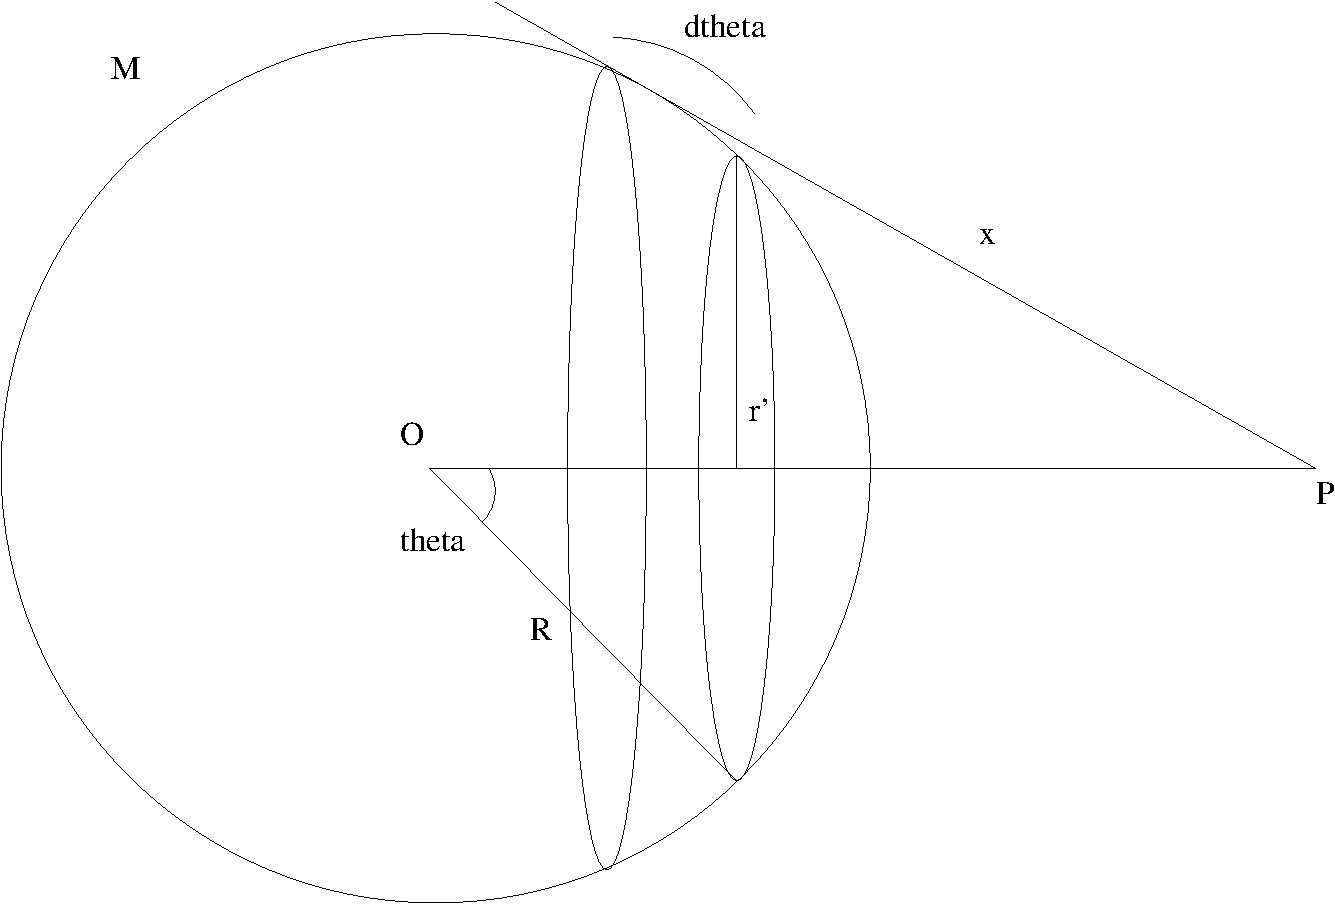
\includegraphics[scale=0.3]{immagini/fisica1/crosta}
\end{figure}
\[F=G\frac{Mm}{r^2}\]
\[r'=R\sin\theta\qquad \ud A=2\pi r'R\ud\theta\]
\[\frac{\ud m}{M}=\frac{\ud
A}{4\pi R^2}=\frac{2\pi r'R\ud\theta}{4\pi
R^2}=\frac{R\sin\theta\ud\theta}{2R}=\frac{\sin\theta\ud\theta}{2}\]
\[\ud m=\frac{M\sin\theta\ud\theta}{2}\]
\[U=-\frac{Gmm'}{r}\qquad\ud U=-\frac{G\ud m m'}{x}\]
\[x^2=R^2+r^2-2rR\cos\theta\]
Derivando a sinistra in $x$ e a destra in $\theta$ si ha:
\[2x\,\ud x=2rR\sin\theta\ud\theta\sin\theta\ud\theta\]
\[\sin\theta\ud\theta=\frac{x\ud x}{rR}\]
\begin{align*}
U&=-\int_{\text{palla}}\frac{Gm'}{x}\,\ud
m=-\int_{\text{palla}}\frac{Gm'}{x}\frac{M\sin\theta\ud\theta}{2}=-\frac{Gm'
m}{2}\int_{\text{palla}}\frac{\sin\theta}{x}\ud\theta\\
&=-\frac{Gmm'}{2rR}\int\frac{x}{x}\ud
x=-\frac{Gmm'}{2rR}\int_{r-R}^{r+R}\ud
x=-\frac{Gmm'}{2rR}[r+R-r+r]\\
&=-\frac{Gmm'}{2rR}2R=-\frac{Gmm'}{r}
\end{align*}
Possiamo quindi concentrare tutta la massa nel centro della palla (se $P$ sta fuori).
Se $P$ è esterno: 
\[U=-\frac{Gmm'}{r}\qquad F=-\frac{\ud U}{\ud
r}=\frac{Gmm'}{r^2}\]
Se $P$ è interno vale il discorso precedente fino alla scelta degli
estremi:
\begin{align*}
U(P)&=-\frac{Gmm'}{2rR}\int_{R-r}^{r+R}\ud x=-\frac{Gmm'}{2rR}[r+R-R+r]\\
&=-\frac{Gmm'}{2rR}2r=-\frac{Gmm^2}{R}=\const
\end{align*}
\[\ve F=-\frac{\ud U}{\ud \ve r}=0\]

Quindi un punto all'interno del guscio non risente di alcuna
forza, questo lo si può dimostrare ragionando con in coni, in
quanto per ogni cono le forze sono uguali.
\subsection{Caso sfera piena}
All'esterno:
\[F=-G\frac{Mm'}{r^2}\]
Dentro:
\[F=-G\frac{M^{\text{int}}m'}{r^2}\]
\[\frac{M^{\text{int}}}{M^{\text{tot}}}=\frac{V^{\text{int}}}{V^{\text{tot}}}=\frac{\frac{4}{3}\pi r^2\rho}{\frac{4}{3}\pi R^3\rho}\]
\[M^{\text{int}}=\frac{r^3}{R^3}M^{\text{tot}}\]
\[F=-\frac{Gr^3M^{\text{tot}}m'}{r^2R^3}=-\frac{Gmm'r}{R^3}=-kr\]
ha l'espressione di una forza elastica.

\begin{Es}[posta pneumatica interterrestre]
Immaginiamo di fare un buco che attraversa tutta la terra, passando per il centro. Un pacco lanciato al suo interno sarebbe sottoposto ad una forza del tipo:
\[F=-kr\qquad k=\left(G\frac{m'M_T}{R_T^3}\right)\]
\[T=2\pi\sqrt{\frac{m'}{k}}=2\pi\sqrt{\frac{R_T^3}{GM_T}}=2\pi\sqrt{\frac{R_T}{g}}\simeq \SI{40}{\minute} \]
\end{Es}
\section{Interpretazione delle leggi di Keplero}
\subsection{Seconda legge}

L'unica ipotesi che utilizziamo è che la forza sia centrale,
quindi il risultato è estendibile a tutte le forze centrali. Una
forza si dice centrale quando è diretta come la congiungente dei
due punti che interagiscono.

\begin{figure}[htbp]
   \centering
   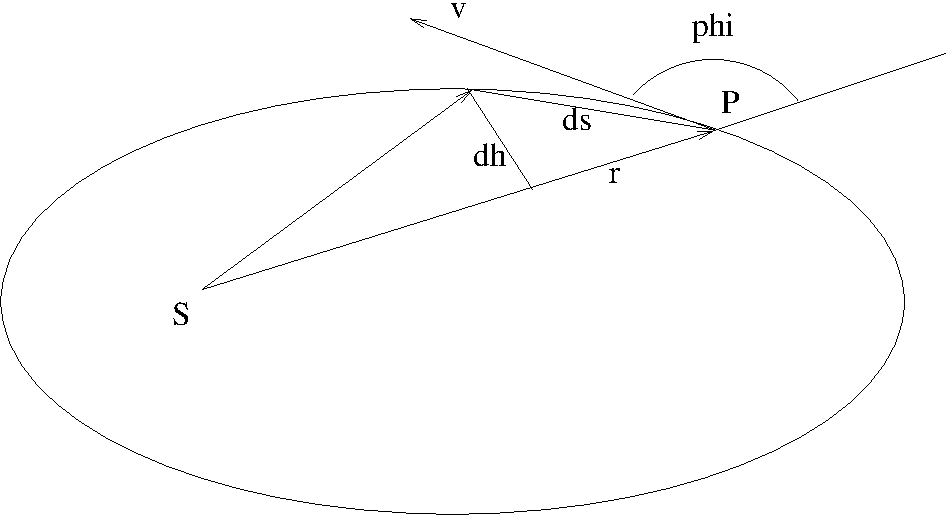
\includegraphics[scale=0.45]{immagini/fisica1/keplero}
\end{figure}



\[
\frac{\ud\ve L_S}{\ud t}=\ve\tau_S=0\quad\text{perché }\ve
F\parallel\ve r
\]
\[\ve L_S=\ve r\times m\ve v=\overrightarrow{\const}\]
\[L_S=rmv\sin\phi={\const}\]
\[\ud h=\ud s\sin\phi\]
\index{velocità!areolare}
\[
\text{velocità areolare}=\frac{\ud A}{\ud t}=\frac{r\ud h}{2\ud
t}=\frac{r\sin\phi\ud s}{2\ud t}=\frac{r}{2}v\sin\phi
\]
\[L_S=\frac{\ud A}{\ud t}2m\qquad\frac{\ud A}{\ud
t}=\frac{L_S}{2m}=\const\]
\subsection{Terza legge}
\[F=\frac{GM_Sm}{R^2}=ma=\frac{mv^2}{R}=\omega^2Rm\]
\[\frac{GM_S}{R^2}=\omega^2R\qquad \omega=\frac{2\pi}{T}\]
\[\frac{GM_S}{R^2}=\frac{4\pi^2}{T^2}R\qquad
T^2=\frac{4\pi^2}{GM_S}R^3\]
\[\frac{T^2}{R^3}=\frac{4\pi^2}{GM_S}=\const\]

\section{\index{accelerazione!di gravità}Accelerazione di gravità}
\[\ve g=\frac{\ve F}{m}\]
Sulla Terra: \[g = \frac{G\frac{M_Tm}{R_T^2}}{m}=\frac{GM_T}{R_T^2}\simeq \SI{9.836}{\meter\per\second\squared} \]
In realtà questo valore è variabile, dall'equatore ai poli, cioè
circa tra $9.78\div9.86$, a causa della forza centrifuga e dallo
schiacciamento dei poli. Per quanto riguarda la forza centrifuga
questa è nulla ai poli e massima all'equatore quindi:
\[F_C=m\omega^2R\qquad F_N=mg_{\text{polo}}\]
\[\frac{F_C}{F_N}=\frac{\omega^2R}{g_{\text{polo}}}=\frac{(2\pi)^2}{T^2}\frac{R}{g_{\text{polo}}}\]
\begin{Es}[Satelliti geostazionari]
 I satelliti geostazionari sono satelliti che per il sistema di riferimento della Terra, sono fermi. Questo vuol dire che hanno lo stesso periodo della Terra:
\[
 F = G\frac{Mm}{R^2} = m\frac{v^2}{R}\quad\Rightarrow v=\sqrt{\frac{GM}{R}}
\]
\[
 T = \frac{2 \pi}{\omega} = \frac{2\pi R}{v} = 2\pi R\sqrt{\frac{R}{GM}} = \SI{1}{\dday}
\]
\[
 R = \sqrt[3]{\frac{GMT^2}{4\pi^2}}\simeq \SI{42E3}{\kilo\meter}
\]
quindi l'altitudine sarà $d = R - R_\oplus\simeq \SI{36E3}{\kilo\meter}$.
\end{Es}

\section{\index{bilancia!di torsione}Misurazione della costante di gra\-vi\-ta\-zio\-ne u\-ni\-ver\-sa\-le}
Cavendish con l'articolo ``Misura della massa terrestre'' nel
1798 è il primo a misurare la costante di gravitazione universale
o costante di Cavendish. Cavendish si proponeva di misurare la
massa terrestre e quindi indirettamente $G$.

La bilancia di torsione viene fatta oscillare, il momento è
proporzionale all'angolo di scostamento dalla posizione di
equilibrio, si genera un moto armonico.

\[\tau=-k\theta=I\alpha\qquad\alpha=\frac{\ud^2\theta}{\ud t^2}\]
\[-k\theta=I\ddot\theta\qquad T=2\pi\sqrt\frac{I}{k}\qquad I=2mD^2\]


Da qui sperimentalmente si trova $k$. Avvicinando delle masse più
grosse si genera un momento dovuto alla forza gravitazionale. Si
impone che il momento gravitazionale sia uguale al momento dovuto
alla forza elastica di richiamo.

\[\tau_\text{Newton}=2\frac{GMm}{d^2}D=\tau_\text{torsione}=k\theta\]
\[G=\frac{k\theta d^2}{2MmD}\]
\section{Massa gravitazione e massa inerziale}
Per massa inerziale si intende quella grandezza usata in dinamica
per esempio \mbox{$\ve F=m\ve a$}. Per massa gravitazionale si intende quella usata nella gravitazione per esempio $F=G\frac{Mm}{r^2}$. Anche se la questione è aperta $m_i$ è proporzionale a $m_g$ infatti se $B$ e $C$ sono attratti da $A$ si ha:
\[\frac{F_{BA}}{F_{CA}}=\frac{Gm_{Bg}m_{ag}}{Gm_{Cg}m_{ag}}=\frac{m_{Bg}}{m_{Cg}}=\frac{m_{Bi}a_b}{m_{ci}a_c}\]
\[\text{se }a_C=a_B\Rightarrow\frac{m_{Bg}}{m_{Cg}}=\frac{m_{Bi}}{m_{Ci}}\Rightarrow
m_{Bg}=\frac{m_{Cg}}{m_{Ci}}\cdot m_{Bi}\]
\section{\index{principio!di equivalenza}Principio di equivalenza}
\begin{Pri}[equivalenza di Einstein]
nessun esperimento può rivelare la differenza tra un sistema di riferimento inerziale immerso in un campo gravitazionale $\ve j$ e un sistema non inerziale con accelerazione costante $\ve a=-\ve j$
\end{Pri}
\section{\index{energia!di un'orbita}Energia associata ad un'orbita}
\[E=\frac{1}{2}mv^2-G\frac{Mm}{r^2}=-G\frac{Mm}{2a}\]
\[r(\theta)=\frac{p}{1+e\cos\theta}\]
\[p=\frac{L^2}{m\alpha}\]
\[\alpha=GMm\]
\[e=\text{eccentricità}=\sqrt{1+2^{\frac{EL^2}{m\alpha}}}\]
\[\begin{array}{llc}
e>1&E>0&\text{iperbole}\\
e=1&E=0&\text{parabola}\\
0<e<1&E<0&\text{ellisse}\\
e=0&E<0&\text{circonferenza}\\
\end{array}\]
